\chapter{Regression}

\begin{enumerate}
	
\item Performing the linear regression using \texttt{scipy.stats.linregress} outputs.

\begin{figure}[H]
	\begin{subfigure}[l]{0.2\linewidth}
		\centering
		\begin{tabular}{@{}rr@{}}
			\toprule
			\multicolumn{2}{c}{\texttt{linRegressOutput}} \\
			\midrule
			$\beta_1$     &         1.206366 \\
			$\beta_0$ &         2.463493 \\
			$r$    &         0.985651 \\
			$p$    &         0.000007 \\
			\bottomrule
		\end{tabular}
	\end{subfigure}
	%
	\begin{subfigure}[]{0.8\linewidth}
		\centering
		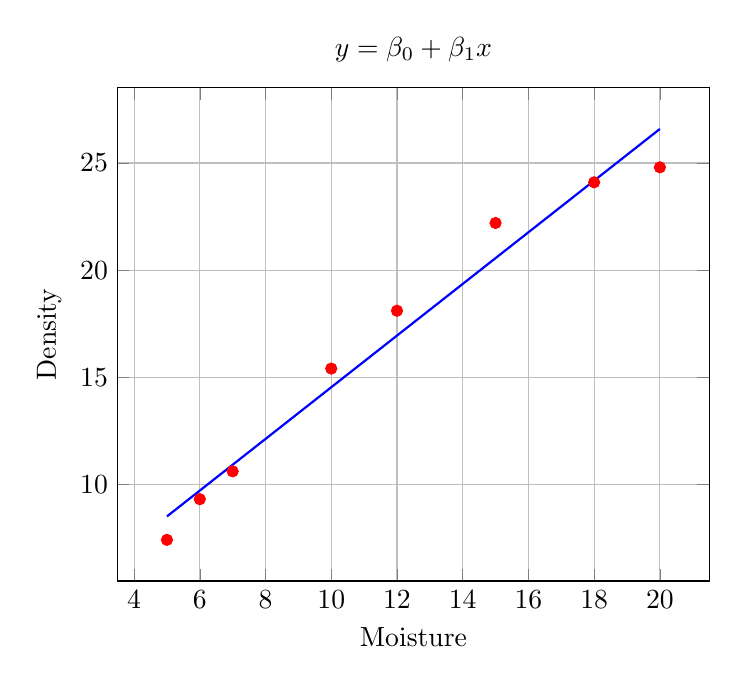
\begin{tikzpicture}
			\begin{axis}[width = 0.75\textwidth,xlabel= Moisture , ylabel= Density , grid=both, title = {$y = \beta_0 + \beta_1 x$}]
				\addplot[thick, smooth, draw=blue][domain= 5 : 20 ]{ 1.2064 *x +  2.4635 };
				\addplot[only marks, color = red] plot coordinates{(5, 7.4) (6, 9.3) (7, 10.6) (10, 15.4) (12, 18.1) (15, 22.2) (18, 24.1) (20, 24.8)};
			\end{axis}
		\end{tikzpicture}
	\end{subfigure}
\end{figure}

\item Performing the linear regression using \texttt{scipy.stats.linregress} outputs.
The value corresponding to $ x = 25 $ is $ y = 147.34 $.

\begin{figure}[H]
	\begin{subfigure}[]{0.2\linewidth}
		\centering
		\begin{tabular}{@{}rr@{}}
			\toprule
			\multicolumn{2}{c}{\texttt{linRegressOutput}} \\
			\midrule
			$\beta_1$     &    -2.376000e+00 \\
			$\beta_0$ &     2.067400e+02 \\
			$r$    &    -9.996792e-01 \\
			$p$    &     1.543680e-07 \\
			\bottomrule
		\end{tabular}
		
	\end{subfigure}
%
\begin{subfigure}[]{0.8\linewidth}
\centering

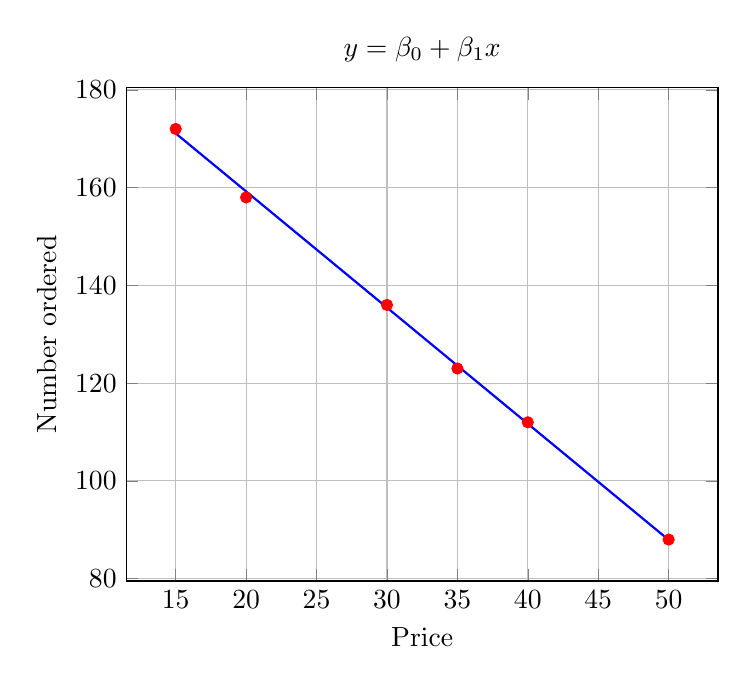
\begin{tikzpicture}
	\begin{axis}[width = 0.75\textwidth,xlabel= Price , ylabel= Number ordered , grid=both, title = {$y = \beta_0 + \beta_1 x$}]
		\addplot[thick, smooth, draw=blue][domain= 15.0 : 50.0 ]{ -2.376 *x +  206.74 };
		\addplot[only marks, color = red] plot coordinates{(50.0, 88.0) (40.0, 112.0) (35.0, 123.0) (30.0, 136.0) (20.0, 158.0) (15.0, 172.0)};
	\end{axis}
\end{tikzpicture}
	\end{subfigure}
\end{figure}

\item Performing the linear regression using \texttt{scipy.stats.linregress} outputs.
The value corresponding to $ x = 3.2 $ is $ y = 0.04476 $.

\begin{figure}[H]
	\begin{subfigure}[]{0.2\linewidth}
		\centering
		\begin{tabular}{@{}rr@{}}
			\toprule
			\multicolumn{2}{c}{\texttt{linRegressOutput}} \\
			\midrule
			$\beta_1$     &         0.011743 \\
			$\beta_0$ &         0.007186 \\
			$r$    &         0.995607 \\
			$p$    &         0.000029 \\
			\bottomrule
		\end{tabular}
		
	\end{subfigure}
	%
	\begin{subfigure}[]{0.8\linewidth}
		\centering
		
		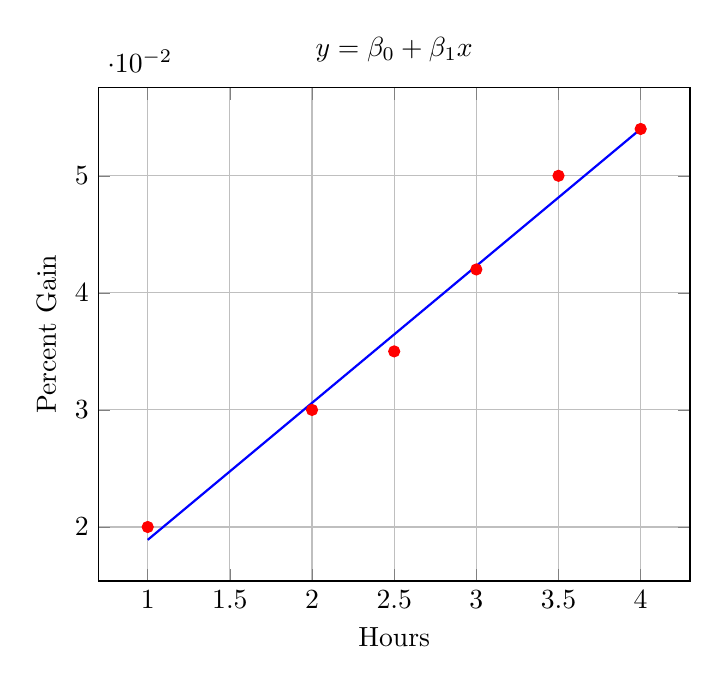
\begin{tikzpicture}
			\begin{axis}[width = 0.75\textwidth,xlabel=Hours, ylabel=Percent Gain, grid=both, title = {$y = \beta_0 + \beta_1 x$}]
				\addplot[thick, smooth, draw=blue][domain=1.0:4.0]{0.0117*x + 0.0072};
				\addplot[only marks, color = red] plot coordinates{(1.0, 0.02) (2.0, 0.03) (2.5, 0.035) (3.0, 0.042) (3.5, 0.05) (4.0, 0.054)};
			\end{axis}
		\end{tikzpicture}
	\end{subfigure}
\end{figure}
	
\item Performing the linear regression using \texttt{scipy.stats.linregress} outputs.
The value corresponding to $ x = 0.43 $ is $ y = 2439.75 $.

\begin{figure}[H]
	\begin{subfigure}[]{0.2\linewidth}
		\centering
		\begin{tabular}{@{}rr@{}}
			\toprule
			\multicolumn{2}{c}{\texttt{linRegressOutput}} \\
			\midrule
			$\beta_1$     &     12245.746692 \\
			$\beta_0$ &     -2825.916824 \\
			$r$    &         0.695796 \\
			$p$    &         0.025447 \\
			\bottomrule
		\end{tabular}
		
	\end{subfigure}
	%
	\begin{subfigure}[]{0.8\linewidth}
		\centering
		
		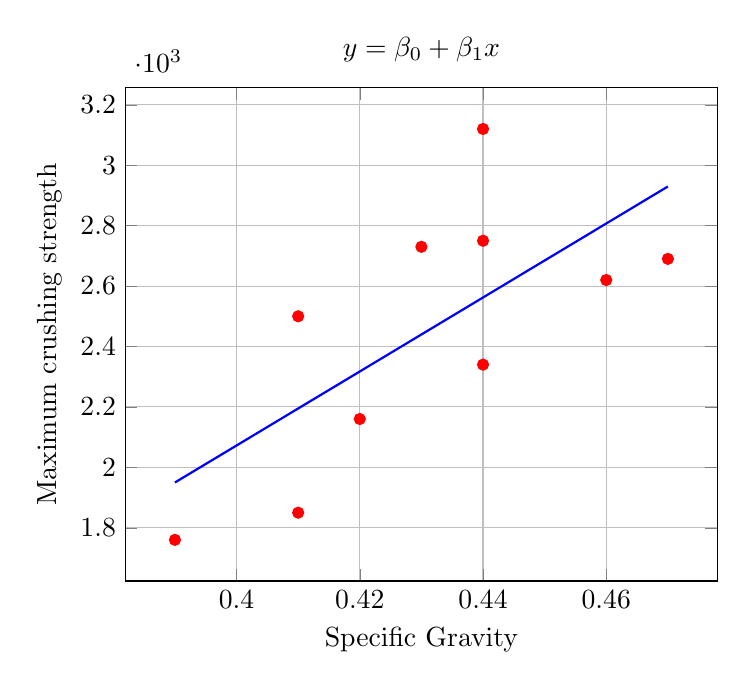
\begin{tikzpicture}
			\begin{axis}[width = 0.75\textwidth,xlabel=Specific Gravity, ylabel=Maximum crushing strength, grid=both, title = {$y = \beta_0 + \beta_1 x$}, scaled y ticks={base 10:-3}]
				\addplot[thick, smooth, draw=blue][domain=0.39:0.47]{12245.7467*x + -2825.9168};
				\addplot[only marks, color = red] plot coordinates{(0.39, 1760.0) (0.41, 1850.0) (0.41, 2500.0) (0.42, 2160.0) (0.43, 2730.0) (0.44, 2340.0) (0.44, 2750.0) (0.44, 3120.0) (0.46, 2620.0) (0.47, 2690.0)};
			\end{axis}
		\end{tikzpicture}
	\end{subfigure}
\end{figure}


\item Performing the linear regression using \texttt{scipy.stats.linregress} outputs.
The least squares estimators are $ A = 2.64 $ and $ B = 11.79 $.
The value corresponding to $ x = 7 $ is $ y = 85.22 $.

\begin{figure}[H]
	\begin{subfigure}[]{0.2\linewidth}
		\centering
		\begin{tabular}{@{}rr@{}}
			\toprule
			\multicolumn{2}{c}{\texttt{linRegressOutput}} \\
			\midrule
			$\beta_1$     &     1.179690e+01 \\
			$\beta_0$ &     2.638928e+00 \\
			$r$    &     9.931055e-01 \\
			$p$    &     9.803790e-09 \\
			\bottomrule
		\end{tabular}
		
	\end{subfigure}
	%
	\begin{subfigure}[]{0.8\linewidth}
		\centering
		
		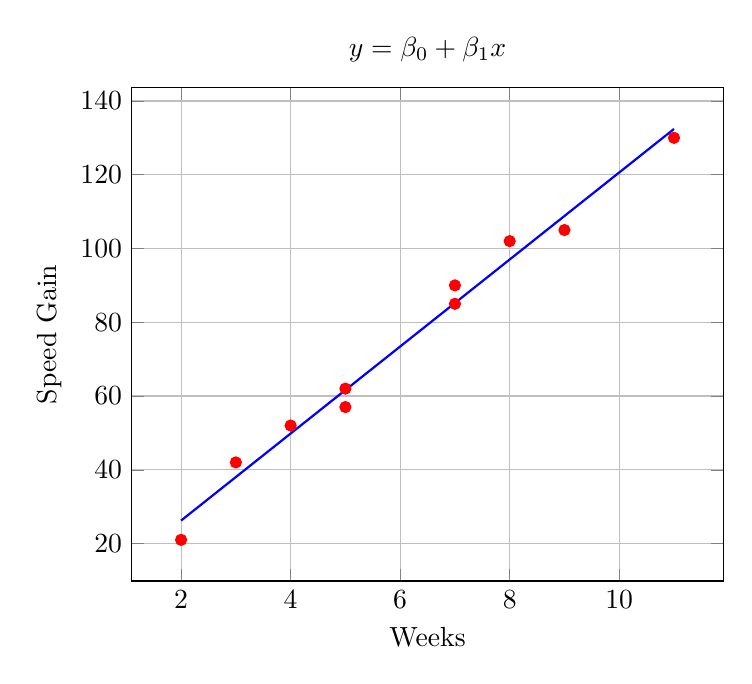
\begin{tikzpicture}
			\begin{axis}[width = 0.75\textwidth,xlabel=Weeks, ylabel=Speed Gain, grid=both, title = {$y = \beta_0 + \beta_1 x$}]
				\addplot[thick, smooth, draw=blue][domain=2.0:11.0]{11.7969*x + 2.6389};
				\addplot[only marks, color = red] plot coordinates{(2.0, 21.0) (3.0, 42.0) (4.0, 52.0) (5.0, 57.0) (5.0, 62.0) (7.0, 85.0) (7.0, 90.0) (8.0, 102.0) (9.0, 105.0) (11.0, 130.0)};
			\end{axis}
		\end{tikzpicture}
	\end{subfigure}
\end{figure}


\item Performing the linear regression using \texttt{scipy.stats.linregress} outputs.
The value corresponding to $ y = 1.15 $ is $ x = 57\% $.

\begin{figure}[H]
	\begin{subfigure}[]{0.2\linewidth}
		\centering
		\begin{tabular}{@{}rr@{}}
			\toprule
			\multicolumn{2}{c}{\texttt{linRegressOutput}} \\
			\midrule
			$\beta_1$     &         0.007026 \\
			$\beta_0$ &         0.749714 \\
			$r$    &         0.997906 \\
			$p$    &         0.000007 \\
			\bottomrule
		\end{tabular}
		
	\end{subfigure}
	%
	\begin{subfigure}[]{0.8\linewidth}
		\centering
		
		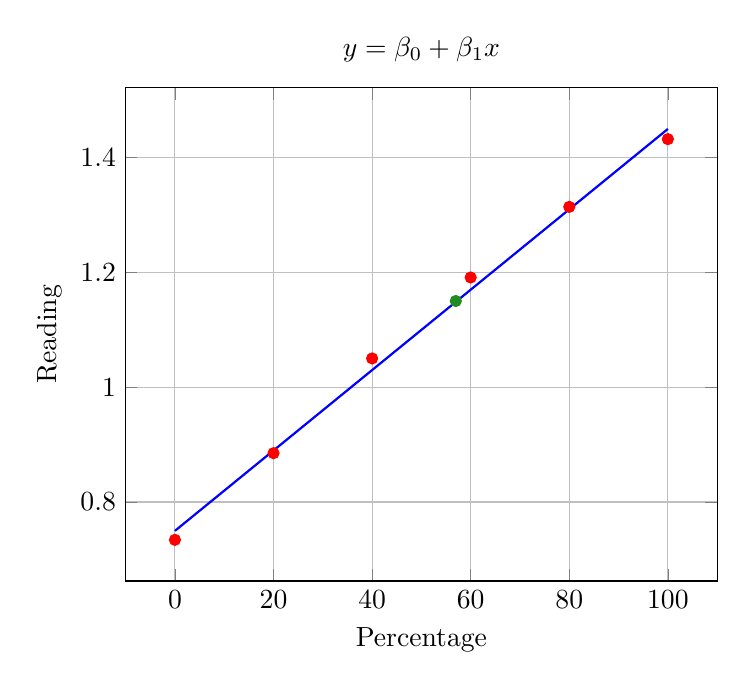
\begin{tikzpicture}
			\begin{axis}[width = 0.75\textwidth,xlabel=Percentage, ylabel=Reading, grid=both, title = {$y = \beta_0 + \beta_1 x$}]
				\addplot[thick, smooth, draw=blue][domain=0.0:100.0]{0.007*x + 0.7497};
				\addplot[only marks, color = red] plot coordinates{(0.0, 0.734) (20.0, 0.885) (40.0, 1.05) (60.0, 1.191) (80.0, 1.314) (100.0, 1.432)};
				\addplot[only marks, color = ForestGreen] plot coordinates{( 56.974379829198845 , 1.15 )};
			\end{axis}
		\end{tikzpicture}
	\end{subfigure}
\end{figure}


\item Performing the linear regression on the first 20 states using \texttt{scipy.stats.linregress} outputs.
The predicted values for the next 5 states are plotted. mean of the first 20 states' math scores is $ \overline{Y} = 525.7 $\\

\begin{figure}[H]
	\begin{subfigure}[]{0.2\linewidth}
		\centering
		\begin{tabular}{@{}rr@{}}
			\toprule
			\multicolumn{2}{c}{\texttt{linRegressOutput}} \\
			\midrule
			$\beta_1$     &    -1.212983e+00 \\
			$\beta_0$ &     5.689428e+02 \\
			$r$    &    -8.640923e-01 \\
			$p$    &     9.078458e-07 \\
			\bottomrule
		\end{tabular}
		
	\end{subfigure}
	%
	\begin{subfigure}[]{0.8\linewidth}
		\centering
		
		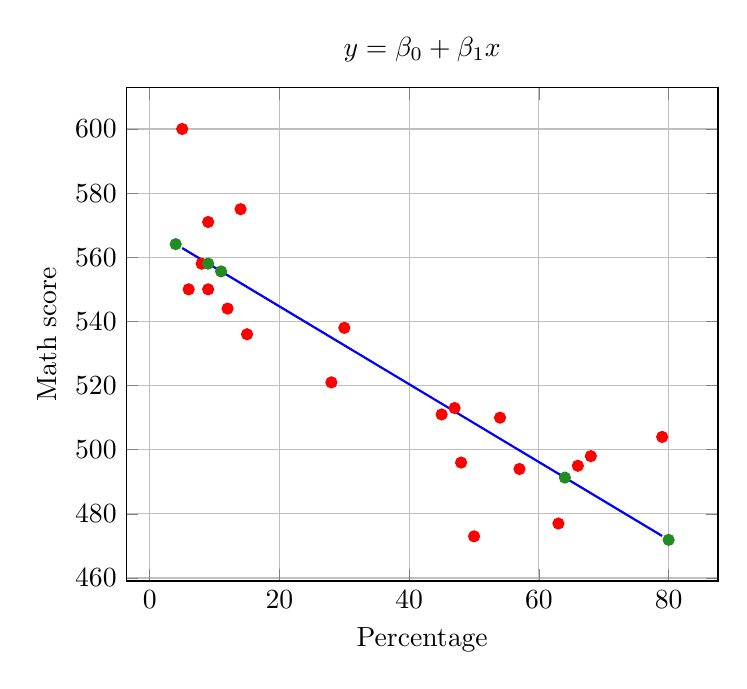
\begin{tikzpicture}
			\begin{axis}[width = 0.75\textwidth,xlabel=Percentage, ylabel=Math score, grid=both, title = {$y = \beta_0 + \beta_1 x$}]
				\addplot[thick, smooth, draw=blue][domain=5:79]{-1.213*x + 568.9428};
				\addplot[only marks, color = red] plot coordinates{(8, 558) (47, 513) (28, 521) (6, 550) (45, 511) (30, 538) (79, 504) (66, 495) (50, 473) (48, 496) (63, 477) (54, 510) (15, 536) (14, 575) (57, 494) (5, 600) (9, 571) (12, 544) (9, 550) (68, 498)};
				\addplot[only marks, color = ForestGreen] plot coordinates{(64, 491.311935572149) (80, 471.9042096163954) (11, 555.6000278005829) (9, 558.0259935450522) (4, 564.0909079062252)};
			\end{axis}
		\end{tikzpicture}
	\end{subfigure}
\end{figure}

\item Verifying the expression for $ \mathrm{Var}(A) $,

\begin{align}
	\mathrm{Var}(Y_i) &= \sigma^2 \nonumber \\
	%
	\mathrm{Var}(B) &= \frac{\mathrm{Var}\left[\sum (x_i - \overline{x})\ (Y_i - \overline{Y})\right]}{S_{xx}^2} \nonumber \\
	%
	&= \frac{\sum (x_i - \overline{x})^2\ \mathrm{Var}(Y_i - \overline{Y})}{S_{xx}^2} = \frac{\sigma^2}{S_{xx}} \\
	%
	\mathrm{Var}(A) &= \overline{x}^2\ \mathrm{Var}(B) + \frac{\mathrm{Var}\sum y_i}{n^2} + 2\ \mathrm{Cov}\left( \frac{\sum y_i}{n}\ ,\  -B \overline{x} \right) \nonumber \\
	%
	&= \frac{\sigma^2}{n} + \overline{x}^2 \frac{\sigma^2}{S_{xx}} - \frac{2B}{n} \ \mathrm{Cov}\left( \sum y_i\ ,\ B \right) \nonumber \\
	&= \frac{\sum x_i^2}{n}\ \frac{\sigma^2}{S_{xx}}
\end{align}

The covariance term vanishes as shown below.

\begin{align}
	\mathrm{Cov}\left( \sum y_i\ ,\ B \right) &= \sum\limits_{i = 1}^{n} \sum\limits_{j = 1}^{n} \mathrm{Cov}\left( y_i\ ,\ \frac{(x_j - \overline{x})\ y_j}{S_{xx}} \right) \nonumber \\
	%
	&= \frac{\sigma^2}{S_{xx}}\ \sum\limits_{i = 1}^{n} (x_i - \overline{x}) = 0
\end{align}


\item Using the data from Problem 4,

$ \sigma^2 $ = 105660 is a point estimate along with an interval estimate based on the $ \chi^2 $ distribution give by $ [54508, 309327] $\\

\item To prove the relation for $ SS_R $ using the previously defined shorthand notation\\
 $ S_{xx}, S_{YY}, S_{xY} $,

\begin{align}
	SS_R &= \sum (Y_i - A - B x_i)^2 = \sum(Y_i - \overline{Y} + B \overline{x} - B x_i)^2 \\
	%
	&= \sum (Y_i - \overline{Y})^2 + B^2\ \sum (\overline{x} - x_i)^2 + 2B\ \sum (Y_i - \overline{Y})(\overline{x} - x_i) \nonumber \\
	%
	&= S_{YY} + \frac{S_{xY}^2}{S_{xx}} - 2\ \frac{S_{xY}^2}{S_{xx}} \nonumber \\
	%
	&= \frac{S_{xx}S_{YY} - S_{xY}^2}{S_{xx}}
\end{align}

\item Performing the linear regression using \texttt{scipy.stats.linregress} outputs.
Testing the hypothesis that $ \beta_1 = 0 $ gives a p-value of $ 1.6\% $. The hypothesis can be rejected at $ 5\% $ confidence level.


\begin{figure}[H]
	\begin{subfigure}[]{0.2\linewidth}
		\centering
		\begin{tabular}{@{}rr@{}}
			\toprule
			\multicolumn{2}{c}{\texttt{linRegressOutput}} \\
			\midrule
			$\beta_1$     &         0.047795 \\
			$\beta_0$ &        46.466853 \\
			$r$    &         0.626258 \\
			$p$    &         0.016568 \\
			\bottomrule
		\end{tabular}
		
	\end{subfigure}
	%
	\begin{subfigure}[]{0.8\linewidth}
		\centering
		
		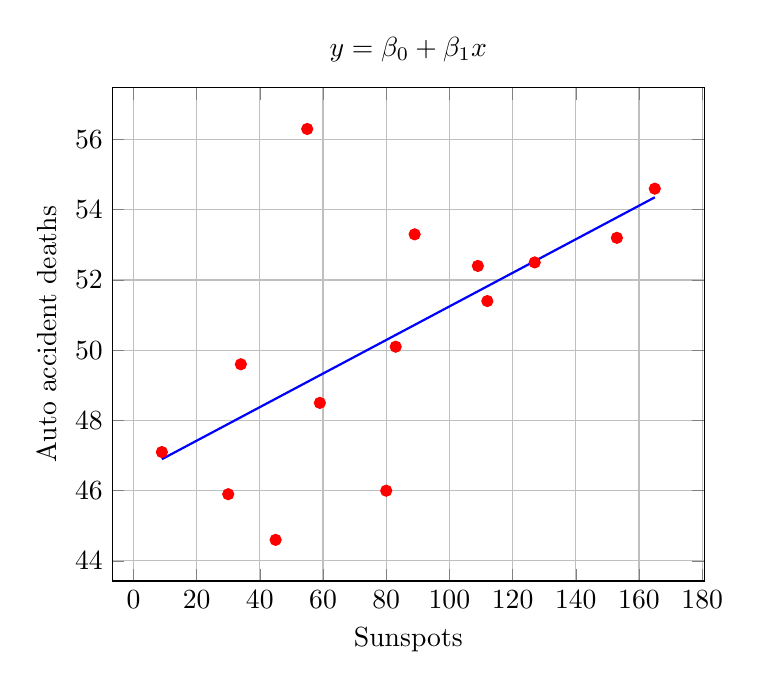
\begin{tikzpicture}
			\begin{axis}[width = 0.75\textwidth,xlabel=Sunspots, ylabel=Auto accident deaths, grid=both, title = {$y = \beta_0 + \beta_1 x$}]
				\addplot[thick, smooth, draw=blue][domain=9:165]{0.0478*x + 46.4669};
				\addplot[only marks, color = red] plot coordinates{(9, 47.1) (30, 45.9) (34, 49.6) (45, 44.6) (55, 56.3) (59, 48.5) (80, 46.0) (83, 50.1) (89, 53.3) (109, 52.4) (112, 51.4) (127, 52.5) (153, 53.2) (165, 54.6)};
			\end{axis}
		\end{tikzpicture}
	\end{subfigure}
\end{figure}

\item Performing the linear regression using \texttt{scipy.stats.linregress} outputs.
Testing the hypothesis that $ \beta_1 = 0 $ gives a p-value of $ 11.1\% $. The hypothesis cannot be rejected at $ 5\% $ confidence level. This means that salary is not related to height.

\begin{figure}[H]
	\begin{subfigure}[]{0.2\linewidth}
		\centering
		\begin{tabular}{@{}rr@{}}
			\toprule
			\multicolumn{2}{c}{\texttt{linRegressOutput}} \\
			\midrule
			$\beta_1$     &         1.457143 \\
			$\beta_0$ &        -4.985714 \\
			$r$    &         0.483846 \\
			$p$    &         0.110981 \\
			\bottomrule
		\end{tabular}
		
	\end{subfigure}
	%
	\begin{subfigure}[]{0.8\linewidth}
		\centering
		
		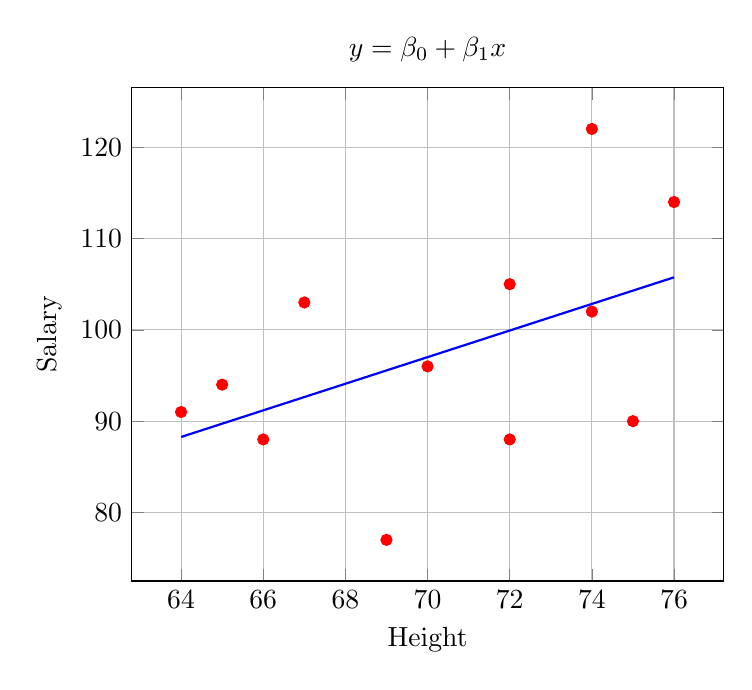
\begin{tikzpicture}
			\begin{axis}[width = 0.75\textwidth,xlabel=Height, ylabel=Salary, grid=both, title = {$y = \beta_0 + \beta_1 x$}]
				\addplot[thick, smooth, draw=blue][domain=64:76]{1.4571*x + -4.9857};
				\addplot[only marks, color = red] plot coordinates{(64, 91) (65, 94) (66, 88) (67, 103) (69, 77) (70, 96) (72, 105) (72, 88) (74, 122) (74, 102) (75, 90) (76, 114)};
			\end{axis}
		\end{tikzpicture}
	\end{subfigure}
\end{figure}

\item Given $ 0 < \beta < 1 $ in a simple linear regression model.

\begin{enumerate}
	\item \begin{align}
		x &< \frac{\alpha}{(1 - \beta)} \to x < \alpha + \beta x \nonumber \\
		%
		\mathbb{E}[Y_i] &= \alpha + \beta x \to \mathbb{E}[Y] > x \nonumber \\
		%
		\mathbb{E}[Y] &< \frac{\alpha}{1 - \beta} \qquad \text{obvious}	\\
		%
		\therefore x &< \mathbb{E}[Y] < \frac{\alpha}{1 - \beta}			
	\end{align}

	\item Same as previous part with all inequalities reversed. This proves that $ \mathbb{E}[Y] $ always lies in between these two values.
	
	\begin{figure}[H]
		\centering
		\begin{tikzpicture}
			\begin{axis}[axis equal, grid = both, grid style={line width=.1pt, draw=gray!30, dashed},
				 width = 0.75\textwidth, xmin = -4, xmax = 8, ymin = -4, ymax = 8, title = {comparing two straight lines with $ y = 0.5x + 1$}]
				\addplot[thick, smooth, draw=red, dashed][name path = f1, domain = -8:10]{x};
				\addplot[thick, smooth, draw=PineGreen, dashed][name path = f1, domain = -8:10]{2};
				\addplot[thick, smooth, draw=blue][name path = f2, domain = -8:10]{0.5*x + 1};
				
				
				\node[color=PineGreen, fill=white] at (axis cs: -3,2) {$ y = \frac{\alpha}{1 - \beta} $};
				\node[color=red, rotate = 45, fill=white] at (axis cs: -2,-2) {$ y = x $};
				\node[color=blue, rotate = 22.5, fill=white] at (axis cs: 6,4) {$ \mathbb{E}[Y] $};
				
							\end{axis}
		\end{tikzpicture}
	\end{figure}

\end{enumerate}

\item Given a linear regression $ Y = 0.159 + 0.4X + e $, with $ e \sim \mathcal{N}(0, \sigma^2) $. The predictions are outlined in the figure below.

\begin{figure}[H]
	\begin{subfigure}[]{0.2\linewidth}
		\centering
		\begin{tabular}{@{}rr@{}}
			\toprule
			$X$     &    $ Y $ \\
			\midrule
			  0.200  &  0.239    \\
			 0.265	&  0.265   \\
			  0.310  &  0.283  \\
			\bottomrule
		\end{tabular}
		
	\end{subfigure}
	%
	\begin{subfigure}[]{0.8\linewidth}
		\centering
		
		\begin{tikzpicture}
			\begin{axis}[axis equal, width = 0.75\textwidth, xlabel=First Year Average, ylabel=Second Year Average, grid=both, title = {$y = 0.159 + 0.4 x$}]
				\addplot[thick, smooth, draw=blue][domain=0:0.4]{0.159 + 0.4*x};
				\addplot[thick, smooth, draw=red, dashed][name path = f1, domain = 0:0.4]{x};
				\addplot[only marks, color = ForestGreen] plot coordinates{(0.2, 0.239) (0.265, 0.265) (0.31, 0.283)};
			\end{axis}
		\end{tikzpicture}
	\end{subfigure}
\end{figure}

\item This is a case of gambler's fallacy. When successive events are independent, it is possible merely through chance for successive outcomes to be good or bad without any causal effect of one outcome on the next. For example, tossing a coin 10 times can result in 10 heads just by chance.

\item In order to rearrange the estimator $ A $ of the regression parameter $ \alpha $ into a t-RV with $ n-2 $ DOF,

\begin{align}
	A &\sim \mathcal{N}\left(\alpha\ ,\ \frac{\sigma^2}{S_{xx}}\ \frac{\sum x_i^2}{n}\right) \nonumber \\
	%
	\frac{(A - \alpha)}{\sigma} \sqrt{\frac{nS_{xx}}{\sum x_i^2}} &\sim Z \\ 
	%
	\frac{SS_R}{\sigma^2} &\sim \chi^2_{n-2} \nonumber \\
	%
	\frac{1}{\sigma} \sqrt{\frac{SS_R}{n-2}} &\sim \sqrt{\frac{\chi^2_{n-2}}{(n-2)}}
\end{align}

Rearranging into a t-RV proves the result.

\begin{align}
	t_{n-2} &\sim \frac{Z}{\sqrt{\chi^2_{n-2} / (n-2)}} \nonumber \\
	%	
	t_{n-2} &\sim (A - \alpha)\ \sqrt{\frac{n(n-2)S_{xx}}{SS_R \sum x_i^2}}
\end{align}

\item Performing the linear regression using \texttt{scipy.stats.linregress} outputs.
The value corresponding to $ x = 24 $ is $ y = 12.604 $.

\begin{figure}[H]
	\begin{subfigure}[]{0.2\linewidth}
		\centering
		\begin{tabular}{@{}rr@{}}
			\toprule
			\multicolumn{2}{c}{\texttt{linRegressOutput}} \\
			\midrule
			$\beta_1$     &     5.528289e-01 \\
			$\beta_0$ &    -6.639400e-01 \\
			$r$    &     9.840458e-01 \\
			$p$    &     2.780621e-07 \\
			\bottomrule
		\end{tabular}
		
	\end{subfigure}
	%
	\begin{subfigure}[]{0.8\linewidth}
		\centering
		
		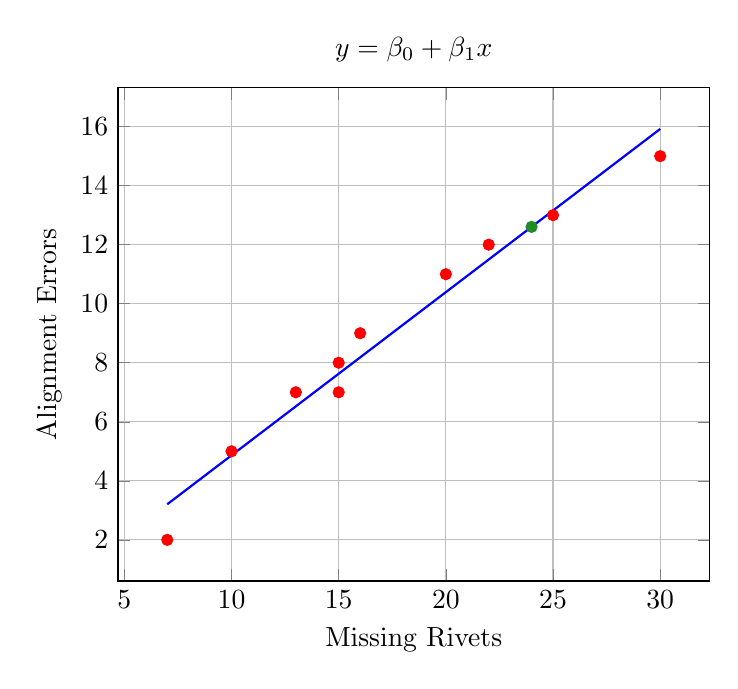
\begin{tikzpicture}
			\begin{axis}[width = 0.75\textwidth,xlabel=Missing Rivets, ylabel=Alignment Errors, grid=both, title = {$y = \beta_0 + \beta_1 x$}]
				\addplot[thick, smooth, draw=blue][domain=7:30]{0.5528*x + -0.6639};
				\addplot[only marks, color = red] plot coordinates{(7, 2) (10, 5) (13, 7) (15, 7) (15, 8) (16, 9) (20, 11) (22, 12) (25, 13) (30, 15)};
				\addplot[only marks, color = ForestGreen] plot coordinates{ (24, 12.603953646898432) };
			\end{axis}
		\end{tikzpicture}
	\end{subfigure}
\end{figure}

Hypothesis testing with $ \gamma = 10\% $ for $ H_0 : \alpha = 1 $ gives a p-value of $ 3.46\% $. This means that the hypothesis can be rejected.

\begin{align}
	H_0 : \alpha = 1 \qquad &\text{vs.} \qquad H_1 : \alpha \neq 1 \nonumber \\
	%
	\text{reject $ H_0 $ if } \qquad & \sqrt{\frac{n(n-2) S_{xx}}{SS_R\ \sum x_i^2}}\ |A - \alpha| > t_{\gamma/2, n-2} \nonumber \\
	%
	\text{accept $ H_0 $  } \qquad & \text{otherwise}
\end{align}

In order to find a confidence interval for $ x_0 = 24 $, using the above t-test,

\begin{align}
	Y(x_0) &\in A + B x_0 \pm t_{\gamma/2, n-2}\ \sqrt{\left(\frac{SS_R}{n-2}\right)\ \left(\frac{1}{n} + \frac{(x_0  - \overline{x})^2}{S_{xx}}\right)} \nonumber \\
	%
	Y(x_0) &\in 12.604 \pm 0.6196 = [11.98, 13.22]
\end{align}

\item Performing the linear regression using \texttt{scipy.stats.linregress} outputs.

\begin{figure}[H]
	\begin{subfigure}[]{0.2\linewidth}
		\centering
		\begin{tabular}{@{}rr@{}}
			\toprule
			\multicolumn{2}{c}{\texttt{linRegressOutput}} \\
			\midrule
			$\beta_1$     &         0.779935 \\
			$\beta_0$ &     -1047.614887 \\
			$r$    &         0.799131 \\
			$p$    &         0.009766 \\
			\bottomrule
		\end{tabular}
		
	\end{subfigure}
	%
	\begin{subfigure}[]{0.8\linewidth}
		\centering
		
		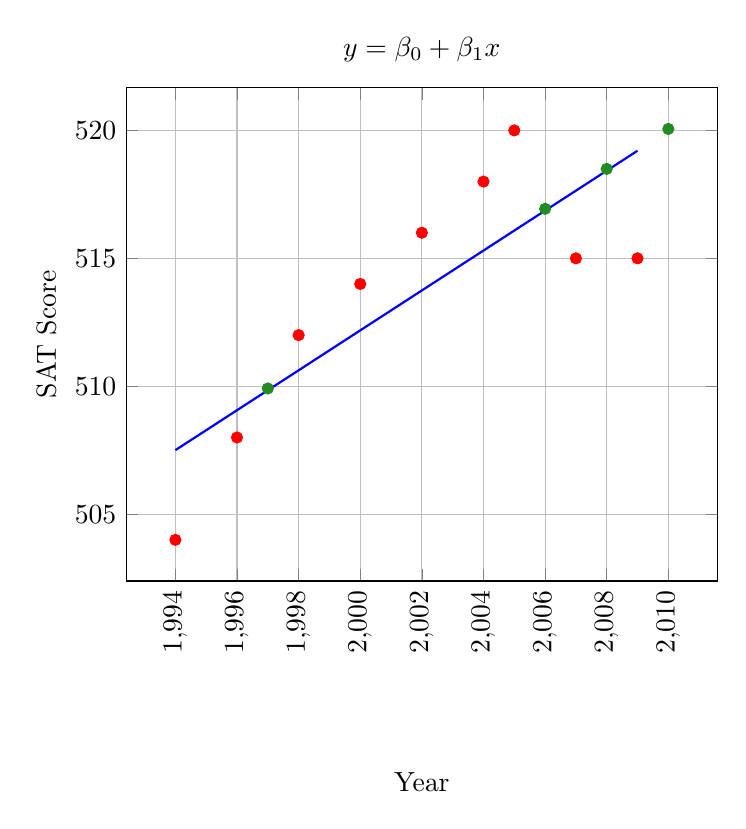
\begin{tikzpicture}
			\begin{axis}[width = 0.75\textwidth,xlabel=Year, ylabel=SAT Score, grid=both, title = {$y = \beta_0 + \beta_1 x$}, xticklabel style ={rotate=90}, xlabel style = {yshift = -0.5in}]
				\addplot[thick, smooth, draw=blue][domain=1994:2009]{0.7799*x + -1047.6149};
				\addplot[only marks, color = red] plot coordinates{(1994, 504) (1996, 508) (1998, 512) (2000, 514) (2002, 516) (2004, 518) (2005, 520) (2007, 515) (2009, 515)};
				\addplot[only marks, color = ForestGreen] plot coordinates{ (1997, 509.91585760517796)(2006, 516.935275080906)(2008, 518.4951456310678)(2010, 520.0550161812296) };
			\end{axis}
		\end{tikzpicture}
	\end{subfigure}
\end{figure}

The predicted values are as tabulated as
\begin{table}[H]
	\centering
	\begin{tabular}{@{}rr@{}}
		\toprule
		$ X $ & $ Y $ \\
		\midrule
		1997     &509.90\\
		2006 &  516.93  \\
		2008    &     518.49 \\
		2010   &  520.05 \\
		\bottomrule
	\end{tabular}
\end{table}

\item Performing the linear regression using \texttt{scipy.stats.linregress} outputs for bladder cancer.
Linear relationship is not very strong with p-value of $ 0.4\% $\\
The value corresponding to $ x = 2500 $ is $ y = 3.96 $.

\begin{figure}[H]
	\begin{subfigure}[]{0.2\linewidth}
		\centering
		\begin{tabular}{@{}rr@{}}
			\toprule
			\multicolumn{2}{c}{\texttt{linRegressOutput}} \\
			\midrule
			$\beta_1$     &         0.001241 \\
			$\beta_0$ &         0.859260 \\
			$r$    &         0.785832 \\
			$p$    &         0.004140 \\
			\bottomrule
		\end{tabular}
		
	\end{subfigure}
	%
	\begin{subfigure}[]{0.8\linewidth}
		\centering
		
		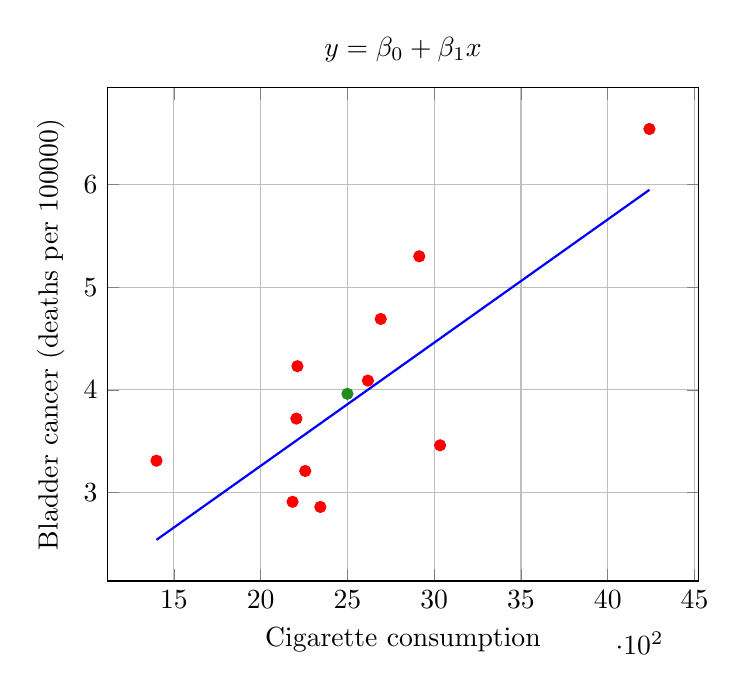
\begin{tikzpicture}
			\begin{axis}[width = 0.75\textwidth,xlabel=Cigarette consumption, ylabel=Bladder cancer (deaths per 100000), grid=both, title = {$y = \beta_0 + \beta_1 x$}, scaled x ticks={base 10:-2}]
				\addplot[thick, smooth, draw=blue][domain=1400:4240]{0.0012*x + 0.8593};
				\addplot[only marks, color = red] plot coordinates{(1400, 3.31) (2184, 2.91) (2206, 3.72) (2212, 4.23) (2257, 3.21) (2344, 2.86) (2618, 4.09) (2692, 4.69) (2914, 5.3) (3034, 3.46) (4240, 6.54)};
				\addplot[only marks, color = ForestGreen] plot coordinates{ (2500, 3.9612972876385455) };
			\end{axis}
		\end{tikzpicture}
	\end{subfigure}
\end{figure}

\item Performing the linear regression using \texttt{scipy.stats.linregress} outputs for lung cancer.
Linear relationship is very strong with p-value of $ 0.67\% $\\
The value corresponding to $ x = 2500 $ is $ y = 3.96 $.

\begin{figure}[H]
	\begin{subfigure}[]{0.2\linewidth}
		\centering
		\begin{tabular}{@{}rr@{}}
			\toprule
			\multicolumn{2}{c}{\texttt{linRegressOutput}} \\
			\midrule
			$\beta_1$     &         0.004715 \\
			$\beta_0$ &         7.443316 \\
			$r$    &         0.759411 \\
			$p$    &         0.006706 \\
			\bottomrule
		\end{tabular}
		
	\end{subfigure}
	%
	\begin{subfigure}[]{0.8\linewidth}
		\centering
		
		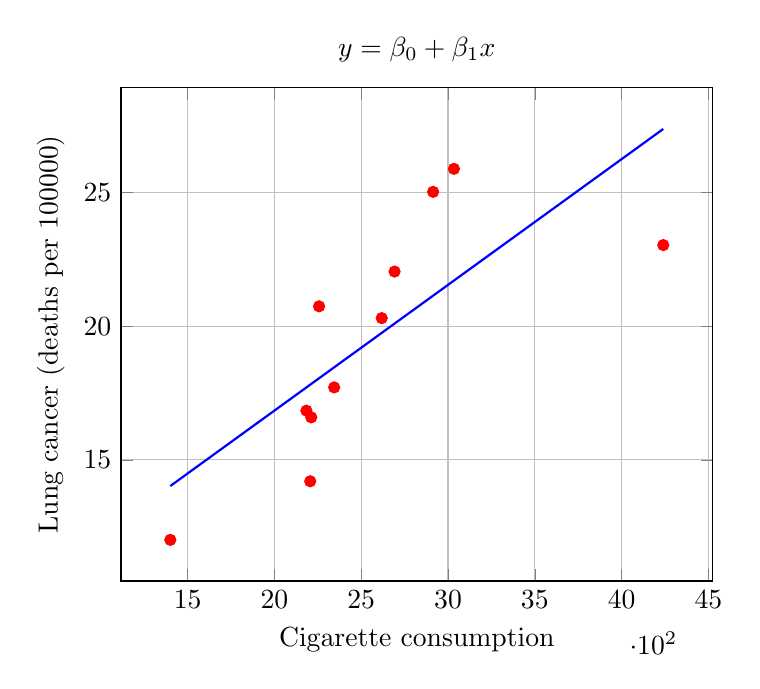
\begin{tikzpicture}
			\begin{axis}[width = 0.75\textwidth,xlabel=Cigarette consumption, ylabel=Lung cancer (deaths per 100000), grid=both, title = {$y = \beta_0 + \beta_1 x$}, scaled x ticks={base 10:-2}]
				\addplot[thick, smooth, draw=blue][domain=1400:4240]{0.0047*x + 7.4433};
				\addplot[only marks, color = red] plot coordinates{(1400, 12.01) (2184, 16.84) (2206, 14.2) (2212, 16.59) (2257, 20.74) (2344, 17.71) (2618, 20.3) (2692, 22.04) (2914, 25.02) (3034, 25.88) (4240, 23.03)};
			\end{axis}
		\end{tikzpicture}
	\end{subfigure}
\end{figure}

\item Performing the linear regression using \texttt{scipy.stats.linregress} outputs for kidney cancer.
Linear relationship is nonexistent with p-value of $ 29\% $\\
The value corresponding to $ x = 2500 $ is $ y = 3.96 $.

\begin{figure}[H]
	\begin{subfigure}[]{0.2\linewidth}
		\centering
		\begin{tabular}{@{}rr@{}}
			\toprule
			\multicolumn{2}{c}{\texttt{linRegressOutput}} \\
			\midrule
			$\beta_1$     &         0.000296 \\
			$\beta_0$ &         2.194573 \\
			$r$    &         0.351066 \\
			$p$    &         0.289780 \\
			\bottomrule
		\end{tabular}
		
	\end{subfigure}
	%
	\begin{subfigure}[]{0.8\linewidth}
		\centering
		
		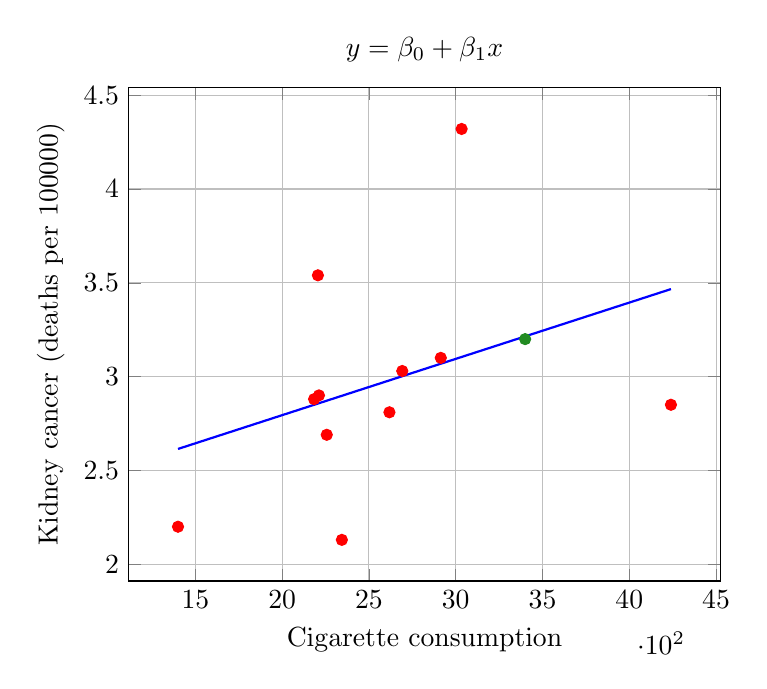
\begin{tikzpicture}
			\begin{axis}[width = 0.75\textwidth,xlabel=Cigarette consumption, ylabel=Kidney cancer (deaths per 100000), grid=both, title = {$y = \beta_0 + \beta_1 x$}, scaled x ticks={base 10:-2}]
				\addplot[thick, smooth, draw=blue][domain=1400:4240]{0.0003*x + 2.1946};
				\addplot[only marks, color = red] plot coordinates{(1400, 2.2) (2184, 2.88) (2206, 3.54) (2212, 2.9) (2257, 2.69) (2344, 2.13) (2618, 2.81) (2692, 3.03) (2914, 3.1) (3034, 4.32) (4240, 2.85)};
				\addplot[only marks, color = ForestGreen] plot coordinates{ (3400, 3.2) };
			\end{axis}
		\end{tikzpicture}
	\end{subfigure}
\end{figure}

The $ 90\% $ confidence interval for the mean death rate with $ x_0 = 3400 $ is given by
$ Y(x_0) = 3.2 \pm 0.52 = [2.67, 3.72] $\\


\item Performing the linear regression using \texttt{scipy.stats.linregress} outputs for leukemia.
Linear relationship is nonexistent with p-value of $ 35.31\% $ for the hypothesis $ H_0 : \beta = 0 $\\
The value corresponding to $ x = 2500 $ is $ y = 3.96 $.
The $ 90\% $ confidence interval for the mean death rate with $ x_0 = 2500 $ is given by
$ Y(x_0) = 6.95 \pm 0.47 = [6.48, 7.42] $\\

\begin{figure}[H]
	\begin{subfigure}[]{0.2\linewidth}
		\centering
		\begin{tabular}{@{}rr@{}}
			\toprule
			\multicolumn{2}{c}{\texttt{linRegressOutput}} \\
			\midrule
			$\beta_1$     &        -0.000371 \\
			$\beta_0$ &         7.877593 \\
			$r$    &        -0.310281 \\
			$p$    &         0.353081 \\
			\bottomrule
		\end{tabular}
		
	\end{subfigure}
	%
	\begin{subfigure}[]{0.8\linewidth}
		\centering
		
		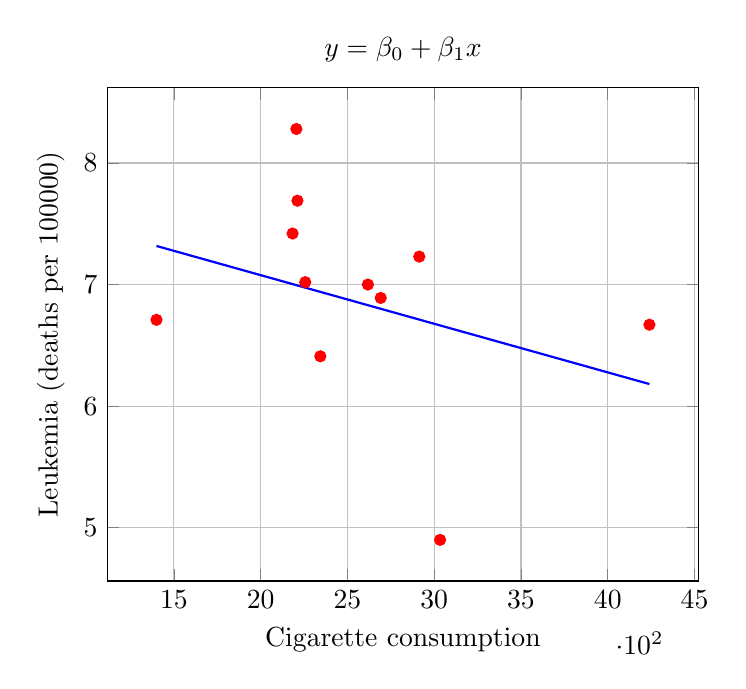
\begin{tikzpicture}
			\begin{axis}[width = 0.75\textwidth,xlabel=Cigarette consumption, ylabel=Leukemia (deaths per 100000), grid=both, title = {$y = \beta_0 + \beta_1 x$}, scaled x ticks={base 10:-2}]
				\addplot[thick, smooth, draw=blue][domain=1400:4240]{-0.0004*x + 7.8776};
				\addplot[only marks, color = red] plot coordinates{(1400, 6.71) (2184, 7.42) (2206, 8.28) (2212, 7.69) (2257, 7.02) (2344, 6.41) (2618, 7.0) (2692, 6.89) (2914, 7.23) (3034, 4.9) (4240, 6.67)};
			\end{axis}
		\end{tikzpicture}
	\end{subfigure}
\end{figure}

\item The variances along with the $ 95\% $ confidence intervals are as follows,

The predicted values are as tabulated as
\begin{table}[H]
	\centering
	\begin{tabular}{@{}lrr@{}}
		\toprule
		Disease		& $ \sigma^2 $	& Interval \\
		\midrule
		Bladder Cancer	& 0.54	& [0.2538, 1.7884]\\
		Lung Cancer	& 9.18	& [4.3436, 30.5983]\\
		Kidney Cancer	& 0.35	& [0.1656, 1.1667]\\
		Leukemia	& 0.73	& [0.3445, 2.4270]\\
		\bottomrule
	\end{tabular}
\end{table}

The variance for the two sets of data are $ \sigma_1^2 = 6.56 $ and $ \sigma_2^2 = 9.02 $. Since the two variances can be arranged into $ \chi^2 $ RVs, their ratio is an f-RV and this can be used to perform the significance test.

\begin{align}
	\frac{SS_{R1}}{\sigma_1^2}\ \frac{\sigma_2^2}{SS_{R2}} &\sim \frac{\chi^2_{n-2}}{\chi^2_{m-2}} \nonumber \\
	%
	\frac{SS_{R1}}{\sigma_1^2}\ \frac{\sigma_2^2}{SS_{R2}}\ \frac{m-2}{n-2} &\sim f_{n-2, m-2}
\end{align}

Using the above f-test, the p-value for equality of the two variances is $ 95.78\% $. This is sufficient to reject the alternative hypothesis at the $ 5\% $ confidence level.

\item Plotting standardized residuals shows that the assumption of linearity is reasonable. There are no discernible trends among the residual data points.

\begin{figure}[H]
	\centering
	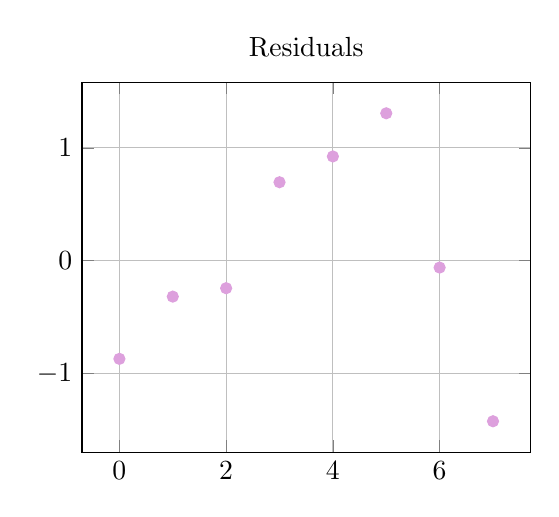
\begin{tikzpicture}
		\begin{axis}[width = 0.6\textwidth, grid=both, title = {Residuals}]
			\addplot[only marks, color = Plum] plot coordinates{(0, -0.8718640529850565) (1, -0.3197402889509025) (2, -0.24520896212952864) (3, 0.6947736741537625) (4, 0.9234350673319759) (5, 1.3062265268670226) (6, -0.06215428337811557) (7, -1.4254676809091682)};
		\end{axis}
	\end{tikzpicture}
\end{figure}

\item $ R = r^2 = 0.999625 $.
p-value is so small for the linear regression that non-linearity can be strongly rejected, although there is a clear pattern in the residuals plot.
The $ 90\% $ confidence interval for the amount of protein with $ x_0 = 1.5 $ is given by
$ Y(x_0) = 41.97 \pm 1.2834 = [40.69, 43.26] $\\

\begin{figure}[H]
	\begin{subfigure}[]{0.2\linewidth}
		\centering
		\begin{tabular}{@{}rr@{}}
			\toprule
			\multicolumn{2}{c}{\texttt{linRegressOutput}} \\
			\midrule
			$\beta_1$     &        38.046693 \\
			$\beta_0$ &       -15.095097 \\
			$r$    &         0.999813 \\
			$p$    &         0.000003 \\
			\bottomrule
		\end{tabular}
		
	\end{subfigure}
	%
	\begin{subfigure}[]{0.8\linewidth}
		\centering
		
		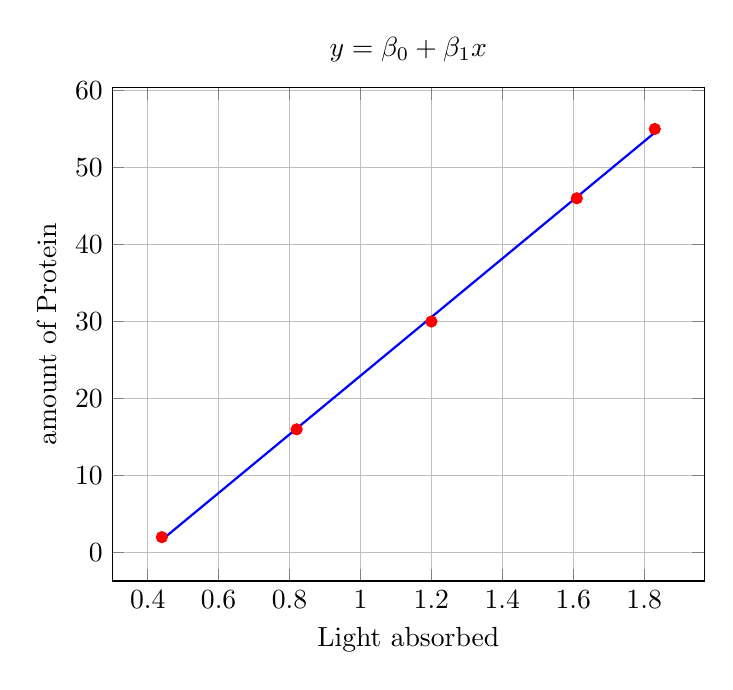
\begin{tikzpicture}
			\begin{axis}[width = 0.75\textwidth,xlabel=Light absorbed, ylabel=amount of Protein, grid=both, title = {$y = \beta_0 + \beta_1 x$}]
				\addplot[thick, smooth, draw=blue][domain=0.44:1.83]{38.0467*x + -15.0951};
				\addplot[only marks, color = red] plot coordinates{(0.44, 2) (0.82, 16) (1.2, 30) (1.61, 46) (1.83, 55)};
			\end{axis}
		\end{tikzpicture}
	\end{subfigure}
\end{figure}

\begin{figure}[H]
	\centering
	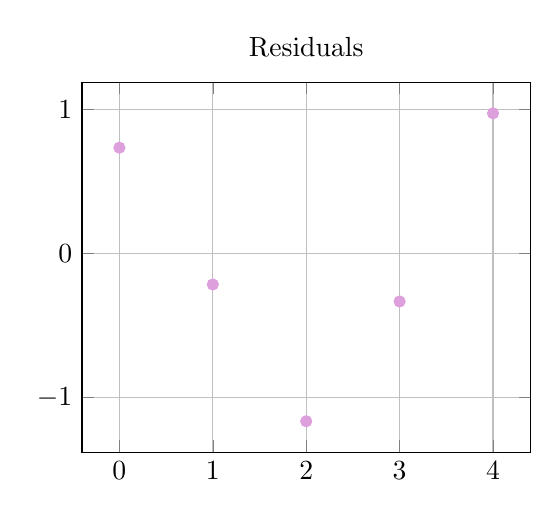
\begin{tikzpicture}
		\begin{axis}[width = 0.6\textwidth, grid=both, title = {Residuals}]
			\addplot[only marks, color = Plum] plot coordinates{(0, 0.7354666946526062) (1, -0.2140537394883921) (2, -1.1635741736293976) (3, -0.3320577240782377) (4, 0.9742189425434361)};
		\end{axis}
	\end{tikzpicture}
\end{figure}	

\item The hypothesis $ H_0 : \beta = 1 $ has a p-value of 2.55\% and thus can be rejected at the 5\% level of significance.

\begin{figure}[H]
	\begin{subfigure}[]{0.2\linewidth}
		\centering
		\begin{tabular}{@{}rr@{}}
			\toprule
			\multicolumn{2}{c}{\texttt{linRegressOutput}} \\
			\midrule
			$\beta_1$     &     9.927803e-01 \\
			$\beta_0$ &    -2.221420e+01 \\
			$r$    &     9.999718e-01 \\
			$p$    &     2.771209e-18 \\
			\bottomrule
		\end{tabular}
		
	\end{subfigure}
	%
	\begin{subfigure}[]{0.8\linewidth}
		\centering
		
		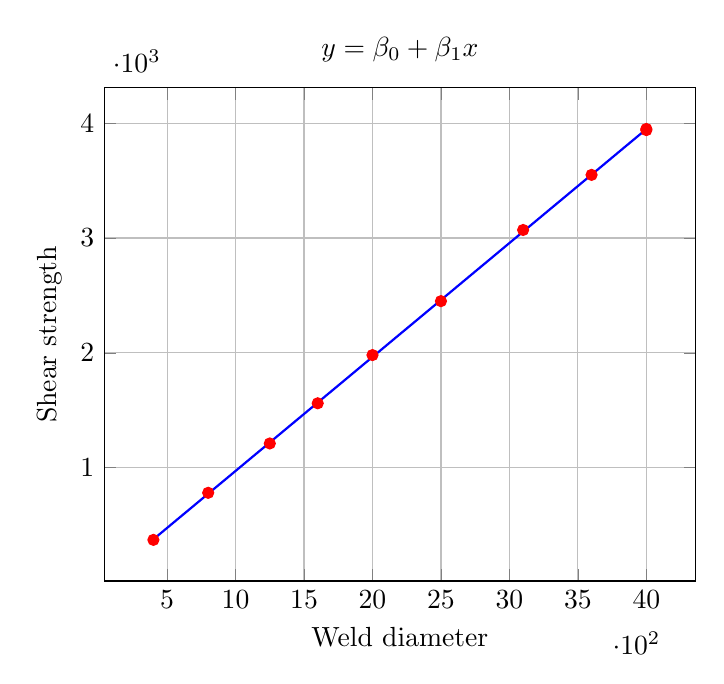
\begin{tikzpicture}
			\begin{axis}[width = 0.75\textwidth,xlabel=Weld diameter, ylabel=Shear strength, grid=both, title = {$y = \beta_0 + \beta_1 x$}, scaled y ticks={base 10:-3}, scaled x ticks={base 10:-2}]
				\addplot[thick, smooth, draw=blue][domain=400:4000]{0.9928*x + -22.2142};
				\addplot[only marks, color = red] plot coordinates{(400, 370) (800, 780) (1250, 1210) (1600, 1560) (2000, 1980) (2500, 2450) (3100, 3070) (3600, 3550) (4000, 3940) (4000, 3950)};
			\end{axis}
		\end{tikzpicture}
	\end{subfigure}
\end{figure}
The expected value for $ y = 2500 $ is $ x = 2459.74 $\\
Plotting the residuals shows no discernible pattern, validating the linear model assumption.
Prediction interval for $ x = 0.2250 $ is $ y = 2211.54 \pm 25.26 = [2186.28, 2236.80] $

\begin{figure}[H]
	\centering
	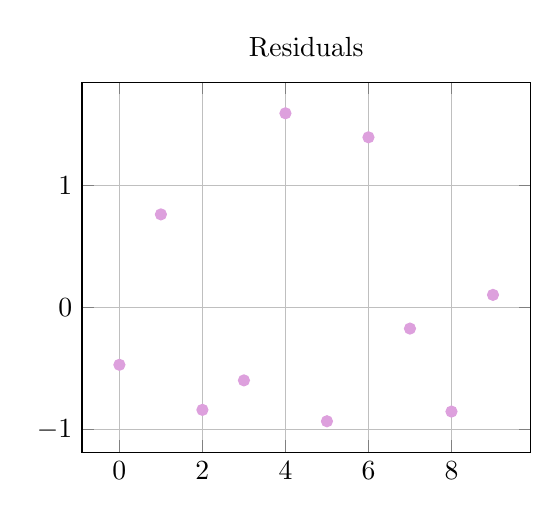
\begin{tikzpicture}
		\begin{axis}[width = 0.6\textwidth, grid=both, title = {Residuals}]
			\addplot[only marks, color = Plum] plot coordinates{(0, -0.4690364067097539) (1, 0.7651373870096277) (2, -0.8389909328923861) (3, -0.597009537982092) (4, 1.5947878838449268) (5, -0.9323952934632576) (6, 1.3976772111696498) (7, -0.17188233803089192) (8, -0.8529558005267355) (9, 0.10466782758088532)};
		\end{axis}
	\end{tikzpicture}
\end{figure}

\item Performing the linear regression using \texttt{scipy.stats.linregress} outputs \\
Prediction interval for $ x = 17 $ is $ y = 179.47 \pm 13.45 = [166.02, 192.92] $\\


\begin{figure}[H]
	\begin{subfigure}[]{0.2\linewidth}
		\centering
		\begin{tabular}{@{}rr@{}}
			\toprule
			\multicolumn{2}{c}{\texttt{linRegressOutput}} \\
			\midrule
			$\beta_1$     &        18.181818 \\
			$\beta_0$ &      -129.618182 \\
			$r$    &         0.908705 \\
			$p$    &         0.000272 \\
			\bottomrule
		\end{tabular}
		
	\end{subfigure}
	%
	\begin{subfigure}[]{0.8\linewidth}
		\centering
		
		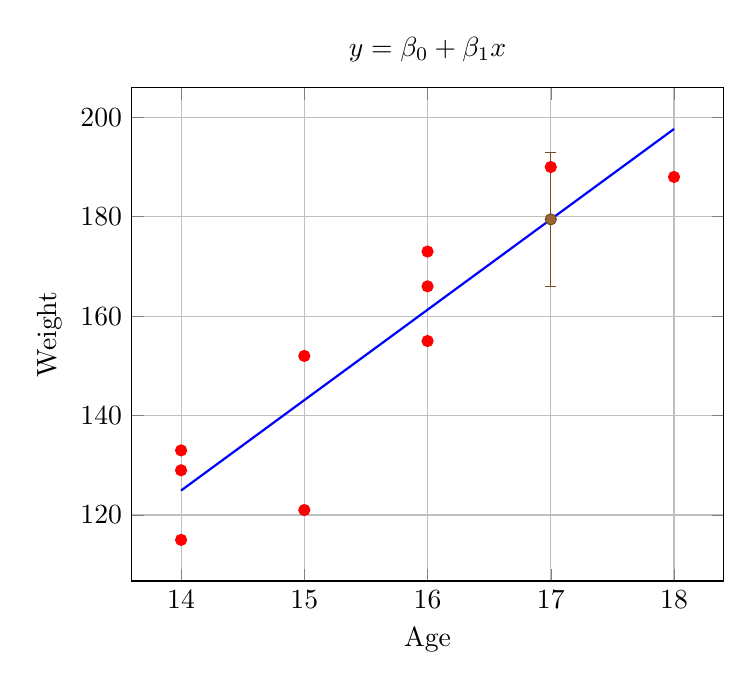
\begin{tikzpicture}
			\begin{axis}[width = 0.75\textwidth,xlabel=Age, ylabel=Weight, grid=both, title = {$y = \beta_0 + \beta_1 x$}]
				\addplot[thick, smooth, draw=blue][domain=14:18]{18.1818*x + -129.6182};
				\addplot[only marks, color = red] plot coordinates{(14, 129) (14, 133) (14, 115) (15, 121) (15, 152) (16, 173) (16, 166) (16, 155) (17, 190) (18, 188)};
				\addplot+[mark = *, error bars/.cd, y dir=both,y explicit] coordinates{ (17, 179.47) +- (0, 13.45) };
			\end{axis}
		\end{tikzpicture}
	\end{subfigure}
\end{figure}

\item Performing the linear regression using \texttt{scipy.stats.linregress} outputs \\
Prediction interval for $ x = 1.52 $ is $ y = 2.5 \pm 0.0089 = [2.4909, 2.5089] $\\

\begin{figure}[H]
	\begin{subfigure}[]{0.2\linewidth}
		\centering
		\begin{tabular}{@{}rr@{}}
			\toprule
			\multicolumn{2}{c}{\texttt{linRegressOutput}} \\
			\midrule
			$\beta_1$     &     4.069680e+00 \\
			$\beta_0$ &    -3.685973e+00 \\
			$r$    &     9.607671e-01 \\
			$p$    &     2.495152e-10 \\
			\bottomrule
		\end{tabular}
		
	\end{subfigure}
	%
	\begin{subfigure}[]{0.8\linewidth}
		\centering
		
		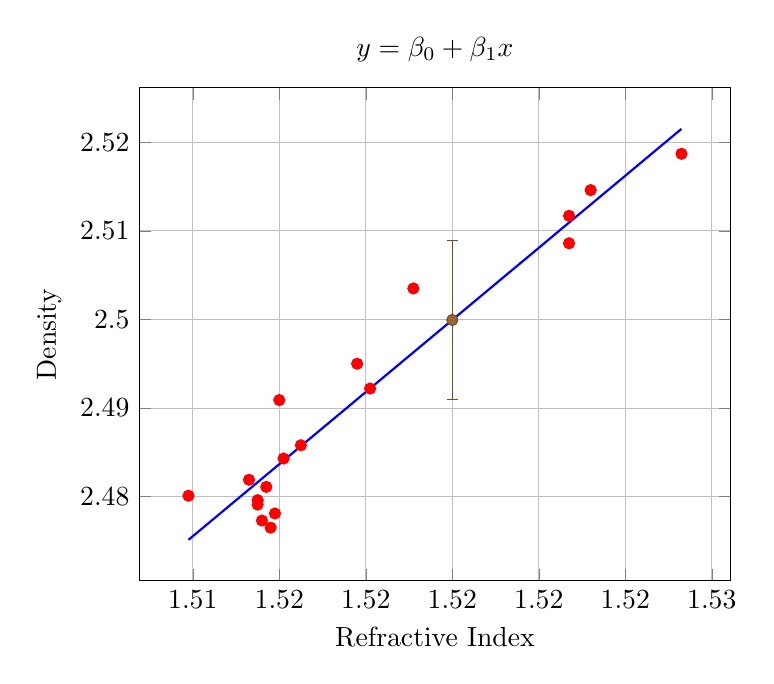
\begin{tikzpicture}
			\begin{axis}[width = 0.75\textwidth,xlabel=Refractive Index, ylabel=Density, grid=both, title = {$y = \beta_0 + \beta_1 x$}]
				\addplot[thick, smooth, draw=blue][domain=1.5139:1.5253]{4.0697*x + -3.686};
				\addplot[only marks, color = red] plot coordinates{(1.5139, 2.4801) (1.5153, 2.4819) (1.5155, 2.4796) (1.5155, 2.4791) (1.5156, 2.4773) (1.5157, 2.4811) (1.5158, 2.4765) (1.5159, 2.4781) (1.516, 2.4909) (1.5161, 2.4843) (1.5165, 2.4858) (1.5178, 2.495) (1.5181, 2.4922) (1.5191, 2.5035) (1.5227, 2.5086) (1.5227, 2.5117) (1.5232, 2.5146) (1.5253, 2.5187)};
				\addplot+[mark = *, error bars/.cd, y dir=both,y explicit] coordinates{ (1.52, 2.4999410235486486) +- (0, 0.00896588582135008)  };
			\end{axis}
		\end{tikzpicture}
	\end{subfigure}
\end{figure}

\item 

\begin{enumerate}
	\item Regression through the origin has the model $ Y = \beta x + e $ where $ e \sim \mathcal{N}(0, \sigma^2) $\\

	\begin{align}
		SS &= \sum\limits_{i = 1}^{n} (Y_i - \widehat{Y_i})^2 = \sum\limits_{i = 1}^{n} (Y_i - Bx_i)^2 \nonumber \\
		%
		\text{differentiating, }\frac{\mathrm{d}}{\mathrm{d}B}\ SS &= 0 \nonumber \\
		%
		0 &= -2 \sum\limits_{i = 1}^{n} x_i  (Y_i - Bx_i) \nonumber \\
		%
		B^* &= \frac{\sum x_i Y_i}{\sum x_i^2}
	\end{align}

	\item  Given the fact that the individual $ Y_i \sim \mathcal{N}(\beta x_i, \sigma^2) $, and $ B $ is a linear combination of the set of $ \{Y_i\} $,

	\begin{align}
		\mathbb{E}[B] &= \frac{1}{\sum x_i^2}\ \sum\limits_{i = 1}^{n} x_i \mathbb{E}[Y_i] \nonumber \\
		%
		&= \frac{1}{\sum x_i^2}\ \beta \sum\limits_{i = 1}^{n} x_i^2 = \beta \\
		%
		\mathrm{Var}(B) &= \frac{\sigma^2 (\sum x_i^2)}{(\sum x_i^2)^2} = \frac{\sigma^2}{\sum x_i^2}
	\end{align}
	
	Thus, B is a normal RV with the above mean and variance.
	
	\item $ SS_R $ is defined as $ \sum (Y_i - Bx_i)^2 $. Each term is the square of a linear combination of normal RVs and thus is also a squared normal RV. This means that $ SS_R $ is a $ \chi^2 $ RV.
	The DOF of this $ \chi^2 $ RV is $ (n-1) $ as one of the $ n $ DOF is lost in determining $ \beta $. Same logic as for the general case of nonzero $ \alpha $.
	
	\item To derive a hypothesis test using the normal RV of $ B $,
	\begin{align}
		H_0 : \beta = \beta_0 \qquad &\text{and} \qquad H_1 : \beta \neq \beta_0 \nonumber \\
		%
		\frac{B - \beta}{\sigma / \sqrt{\sum x_i^2}} \sim Z \qquad &\text{and} \qquad \frac{SS_R}{\sigma^2} \sim \chi^2_{n-1}\\
		%
		\sqrt{\frac{(n-1)\sum x_i^2}{SS_R}} (B - \beta) &\sim t_{n-1} \nonumber \\
		%
		\text{reject $ H_0 $ if } \qquad & \sqrt{\frac{(n-1) \sum x_i^2}{SS_R}}\ |B - \beta_0| > t_{\gamma/2, n-1} \nonumber \\
		%
		\text{accept $ H_0 $  } \qquad & \text{otherwise}
	\end{align}

	\item To find a prediction interval for $ Y(x_0) $,
	
	\begin{align}
		Y - Y_0 &= Y - B x_0 \sim \mathcal{N}\left(0\ ,\  \sigma^2 + \frac{x_0^2 \sigma^2}{\sum x_i^2}\right) 
\nonumber\\
		%
		t_{n-1} &\sim \sqrt{\frac{(n-1)}{SS_R}\ \left(\frac{\sum x_i^2}{\sum x_i^2 + x_0^2}\right)} (Y - B x_0)  \nonumber \\
		%
		Y &\in B x_0 \pm t_{\gamma/2, n-1}\ \sqrt{\frac{SS_R}{(n-1)}\ \left(\frac{\sum x_i^2 + x_0^2}{\sum x_i^2}\right)} 
	\end{align}

	This gives the $ 100 (1 - \gamma)\% $ confidence interval for the prediction $ Y $.

\end{enumerate}

\item Performing the linear regression using \texttt{scipy.stats.linregress} outputs \\
Prediction interval for $ x = 1.52 $ is $ y = 2.5 \pm 0.0089 = [2.4909, 2.5089] $\\


\begin{figure}[H]
	\begin{subfigure}[]{0.2\linewidth}
		\centering
		\begin{tabular}{@{}rr@{}}
			\toprule
			\multicolumn{2}{c}{\texttt{linRegressOutput}} \\
			\midrule
			$\beta_1$     &         1.913991 \\
			$\beta_0$ &        79.248355 \\
			$r$    &         0.866925 \\
			$p$    &         0.005319 \\
			\bottomrule
		\end{tabular}
		
	\end{subfigure}
	%
	\begin{subfigure}[]{0.8\linewidth}
		\centering
		
		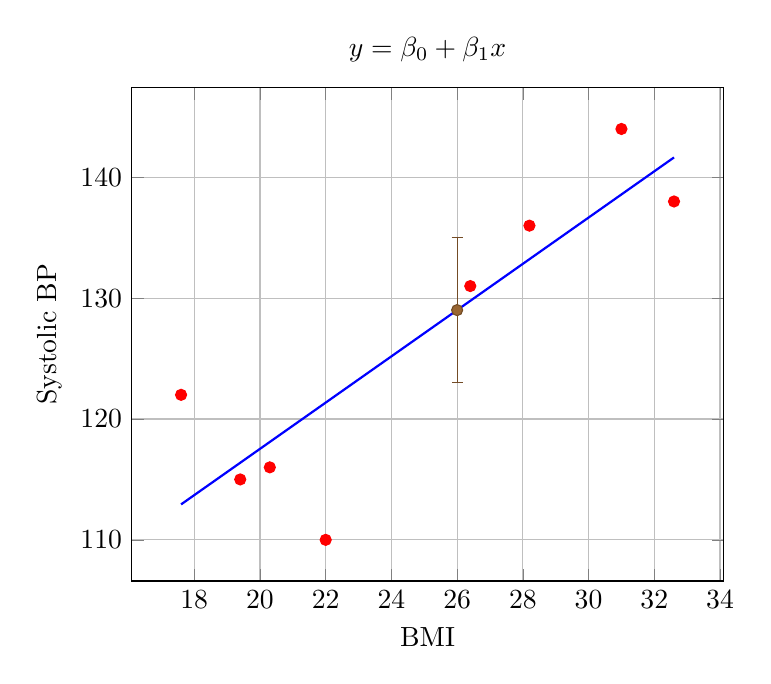
\begin{tikzpicture}
			\begin{axis}[width = 0.75\textwidth,xlabel=BMI, ylabel=Systolic BP, grid=both, title = {$y = \beta_0 + \beta_1 x$}]
				\addplot[thick, smooth, draw=blue][domain=17.6:32.6]{1.914*x + 79.2484};
				\addplot[only marks, color = red] plot coordinates{(17.6, 122) (19.4, 115) (20.3, 116) (22.0, 110) (26.4, 131) (28.2, 136) (31.0, 144) (32.6, 138)};
				\addplot+[mark = *, error bars/.cd, y dir=both,y explicit] coordinates{ (26, 129.012112797972) +- (0, 5.9728)  };
			\end{axis}
		\end{tikzpicture}
	\end{subfigure}
\end{figure}

\item Performing the linear regression using \texttt{scipy.stats.linregress} outputs \\
The hypothesis $ H_0 : \beta_1 = 0 $ has a p-value of $ 0.01\% $ and can be rejected strongly. The Systolic Bp does depend on the Weight.
Mean response interval at $ 95\% $ confidence for $ x = 182 $ is $ y = 144.37 \pm 4.17 = [140.2, 148.53] $\\

\begin{figure}[H]
	\begin{subfigure}[]{0.2\linewidth}
		\centering
		\begin{tabular}{@{}rr@{}}
			\toprule
			\multicolumn{2}{c}{\texttt{linRegressOutput}} \\
			\midrule
			$\beta_1$     &         0.416385 \\
			$\beta_0$ &        68.584433 \\
			$r$    &         0.764442 \\
			$p$    &         0.000087 \\
			\bottomrule
		\end{tabular}
		
	\end{subfigure}
	%
	\begin{subfigure}[]{0.8\linewidth}
		\centering
		
		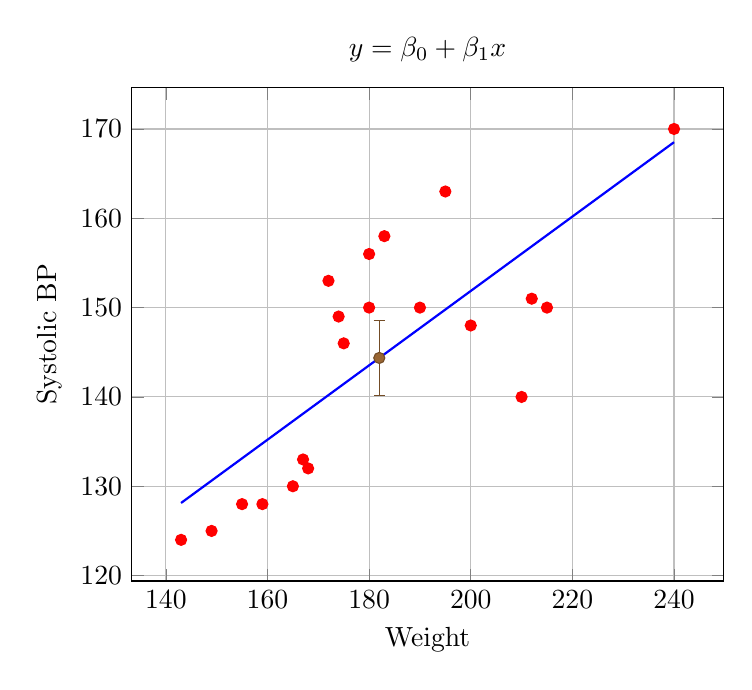
\begin{tikzpicture}
			\begin{axis}[width = 0.75\textwidth,xlabel=Weight, ylabel=Systolic BP, grid=both, title = {$y = \beta_0 + \beta_1 x$}]
				\addplot[thick, smooth, draw=blue][domain=143.0:240.0]{0.4164*x + 68.5844};
				\addplot[only marks, color = red] plot coordinates{(143.0, 124.0) (149.0, 125.0) (155.0, 128.0) (159.0, 128.0) (165.0, 130.0) (167.0, 133.0) (168.0, 132.0) (172.0, 153.0) (174.0, 149.0) (175.0, 146.0) (180.0, 150.0) (180.0, 156.0) (183.0, 158.0) (190.0, 150.0) (195.0, 163.0) (200.0, 148.0) (210.0, 140.0) (212.0, 151.0) (215.0, 150.0) (240.0, 170.0)};
				\addplot+[mark = *, error bars/.cd, y dir=both,y explicit] coordinates{ (182, 144.36655411285548) +- (0, 4.168678497074252)  };
			\end{axis}
		\end{tikzpicture}
	\end{subfigure}
\end{figure}

Plotting the residuals shows no discernible pattern, vindicating the linear model.
The sample correlation coefficient $ r = 0.76444 $\\

\begin{figure}[H]
	\centering
	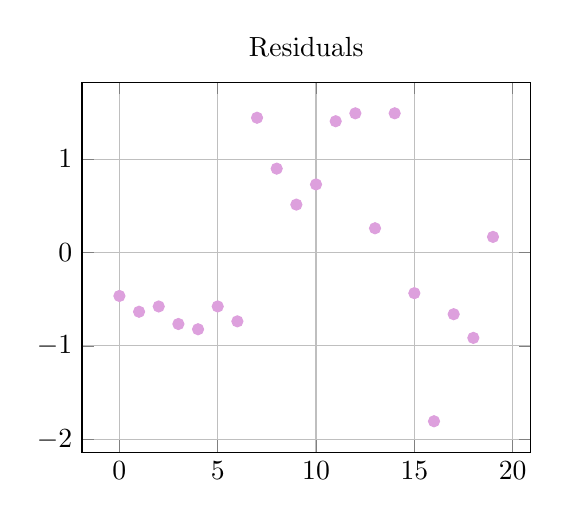
\begin{tikzpicture}
		\begin{axis}[width = 0.6\textwidth, grid=both, title = {Residuals}]
			\addplot[only marks, color = Plum] plot coordinates{(0, -0.46520785627879524) (1, -0.6340804483430937) (2, -0.5775358687038874) (3, -0.7652566539812542) (4, -0.8214206601938011) (5, -0.5771552952772296) (6, -0.7367940774483221) (7, 1.4423654401610952) (8, 0.8976707041154054) (9, 0.5126147502408096) (10, 0.7287981120511084) (11, 1.4050496271616182) (12, 1.4896762099070955) (13, 0.25949614885769146) (14, 1.490056783333755) (15, -0.43522298603922716) (16, -1.806193636046657) (17, -0.6602595843160726) (18, -0.9137587591258486) (19, 0.16715804992564406)};
		\end{axis}
	\end{tikzpicture}
\end{figure}

\item Transforming to linearity,

\begin{align}
	S &= \frac{A}{N^m} \nonumber \\
	%
	\log N &= (1/m)\log A - (1/m)\ \log S \\
	%
	m &= \frac{-1}{\beta_1} = 0.0813 \nonumber \\
	%
	A &= e^{m\beta_0} = 53.91 \nonumber
\end{align}

Performing the linear regression using \texttt{scipy.stats.linregress} outputs \\

\begin{figure}[H]
	\begin{subfigure}[]{0.2\linewidth}
		\centering
		\begin{tabular}{@{}rr@{}}
			\toprule
			\multicolumn{2}{c}{\texttt{linRegressOutput}} \\
			\midrule
			$\beta_1$     &       -12.296305 \\
			$\beta_0$ &        49.031503 \\
			$r$    &        -0.962532 \\
			$p$    &         0.000032 \\
			\bottomrule
		\end{tabular}
		
	\end{subfigure}
	%
	\begin{subfigure}[]{0.8\linewidth}
		\centering
		
		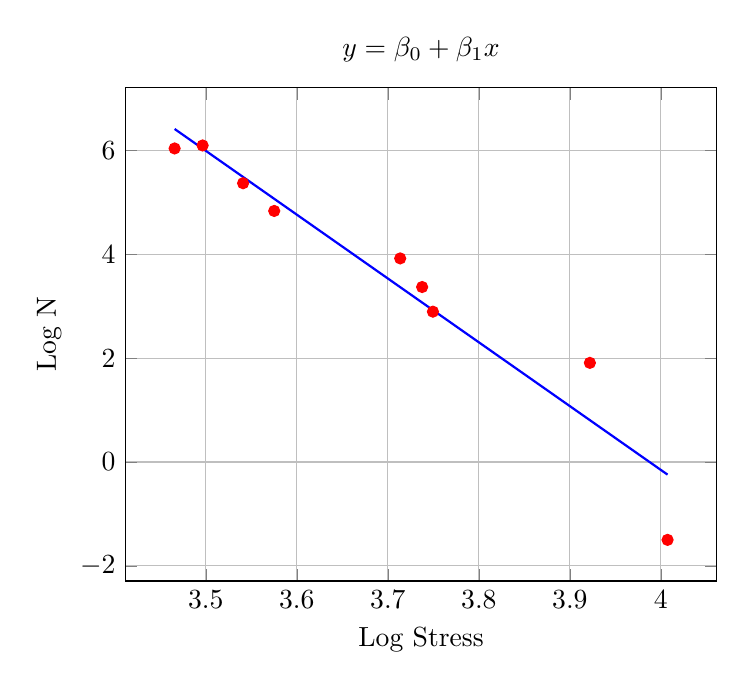
\begin{tikzpicture}
			\begin{axis}[width = 0.75\textwidth,xlabel=Log Stress, ylabel=Log N, grid=both, title = {$y = \beta_0 + \beta_1 x$}]
				\addplot[thick, smooth, draw=blue][domain=3.4657359027997265:4.007333185232471]{-12.2963*x + 49.0315};
				\addplot[only marks, color = red] plot coordinates{(3.4657359027997265, 6.040254711277414) (3.4965075614664802, 6.09807428216624) (3.5409593240373143, 5.3706380281276624) (3.5751506887855933, 4.836281906951478) (3.713572066704308, 3.9219733362813143) (3.7376696182833684, 3.370738174177447) (3.7495040759303713, 2.89591193827178) (3.9219733362813143, 1.9095425048844386) (4.007333185232471, -1.5005835075220182)};
			\end{axis}
		\end{tikzpicture}
	\end{subfigure}
\end{figure}

\item Transforming to linearity,

\begin{align}
	T &= t s^{-n} \nonumber \\
	%
	\log T &= \log t - (n)\ \log s \\
	%
	s &= e^{-\beta_1} = 1.0968 \nonumber \\
	%
	t &= e^{\beta_0} = 22.54 \nonumber
\end{align}

Performing the linear regression using \texttt{scipy.stats.linregress} outputs \\

\begin{figure}[H]
	\begin{subfigure}[]{0.2\linewidth}
		\centering
		\begin{tabular}{@{}rr@{}}
			\toprule
			\multicolumn{2}{c}{\texttt{linRegressOutput}} \\
			\midrule
			$\beta_1$     &        -0.092427 \\
			$\beta_0$ &         3.115315 \\
			$r$    &        -0.967522 \\
			$p$    &         0.000359 \\
			\bottomrule
		\end{tabular}
		
	\end{subfigure}
	%
	\begin{subfigure}[]{0.8\linewidth}
		\centering
		
		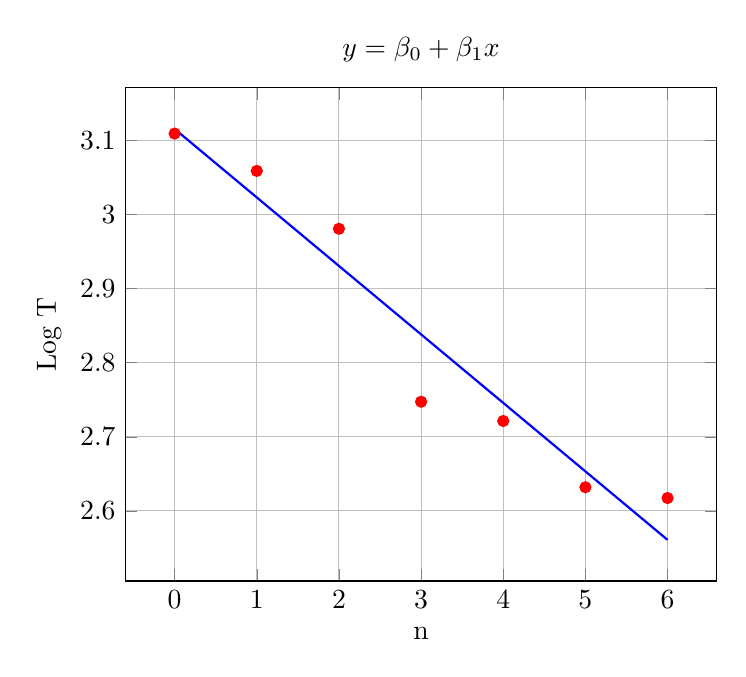
\begin{tikzpicture}
			\begin{axis}[width = 0.75\textwidth,xlabel=n, ylabel=Log T, grid=both, title = {$y = \beta_0 + \beta_1 x$}]
				\addplot[thick, smooth, draw=blue][domain=0.0:6.0]{-0.0924*x + 3.1153};
				\addplot[only marks, color = red] plot coordinates{(0.0, 3.109060958860994) (1.0, 3.0587070727153796) (2.0, 2.9806186357439426) (3.0, 2.747270914255491) (4.0, 2.7212954278522306) (5.0, 2.631888840136646) (6.0, 2.617395832834079)};
			\end{axis}
		\end{tikzpicture}
	\end{subfigure}
\end{figure}

\item Transforming to linearity,

\begin{align}
	Y &= ae^{-bx} \nonumber \\
	%
	\log Y &= \log a - bx \\
	%
	b &= -\beta_1 = 0.0239 \nonumber \\
	%
	a &= e^{\beta_0} = 1.7473 \nonumber
\end{align}

The value corresponding to $ x = 15 $ is $ \log Y = 0.1997 $ and thus $ Y = 1.22 $\\

\begin{figure}[H]
	\begin{subfigure}[]{0.2\linewidth}
		\centering
		\begin{tabular}{@{}rr@{}}
			\toprule
			\multicolumn{2}{c}{\texttt{linRegressOutput}} \\
			\midrule
			$\beta_1$     &        -0.023894 \\
			$\beta_0$ &         0.558096 \\
			$r$    &        -0.871119 \\
			$p$    &         0.023845 \\
			\bottomrule
		\end{tabular}
		
	\end{subfigure}
	%
	\begin{subfigure}[]{0.8\linewidth}
		\centering
		
		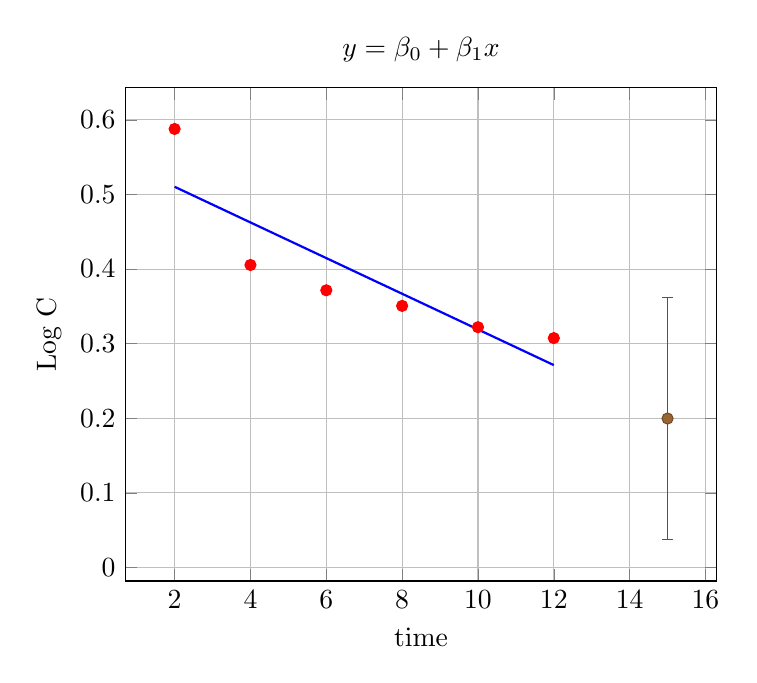
\begin{tikzpicture}
			\begin{axis}[width = 0.75\textwidth,xlabel=time, ylabel=Log C, grid=both, title = {$y = \beta_0 + \beta_1 x$}]
				\addplot[thick, smooth, draw=blue][domain=2.0:12.0]{-0.0239*x + 0.5581};
				\addplot[only marks, color = red] plot coordinates{(2.0, 0.5877866649021191) (4.0, 0.4054651081081644) (6.0, 0.371563556432483) (8.0, 0.35065687161316933) (10.0, 0.3220834991691132) (12.0, 0.3074846997479607)};
				\addplot+[mark = *, error bars/.cd, y dir=both,y explicit] coordinates{ (15, 0.19969019952991002) +- (0, 0.16265365180951408)  };
			\end{axis}
		\end{tikzpicture}
	\end{subfigure}
\end{figure}


\item Transforming to linearity,

\begin{align}
	P &= 1 - e^{-\alpha t} \nonumber \\
	%
	\log (1-P) &= -\alpha t \\
	%
	\alpha &= -\beta_1 = 1.0534 \nonumber
\end{align}

Using the forced pass through origin method from Problem 29,
The value corresponding to $ P = 1/2 $ is $ t = 0.658 $\\

\begin{figure}[H]
	\begin{subfigure}[]{0.2\linewidth}
		\centering
		\begin{tabular}{@{}rr@{}}
			\toprule
			\multicolumn{2}{c}{\texttt{zeroInterceptOutput}} \\
			\midrule
			$\beta_1$     &        -1.0534 \\
			$\beta_0$ &        0 \\
			\bottomrule
		\end{tabular}
		
	\end{subfigure}
	%
	\begin{subfigure}[]{0.8\linewidth}
		\centering
		
		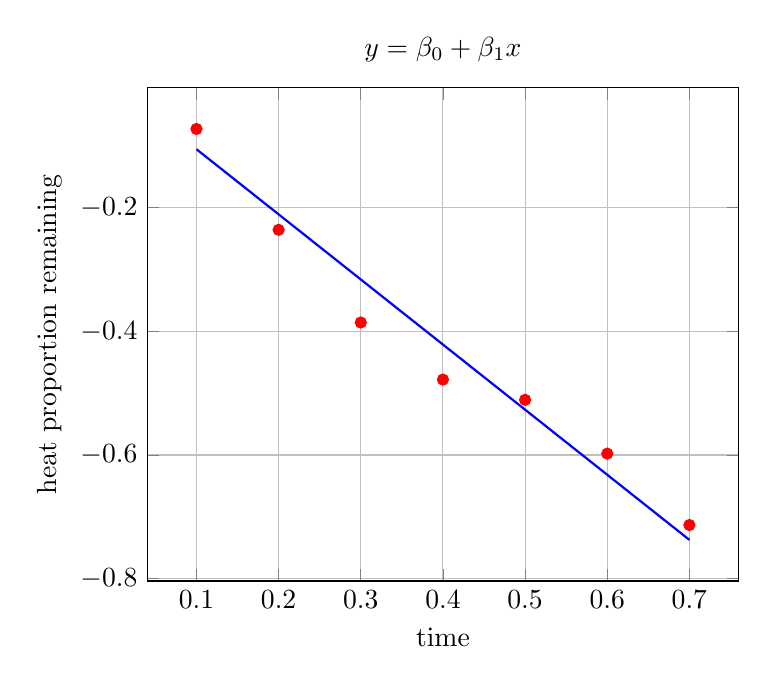
\begin{tikzpicture}
			\begin{axis}[width = 0.75\textwidth,xlabel=time, ylabel=heat proportion remaining, grid=both, title = {$y = \beta_0 + \beta_1 x$}]
				\addplot[thick, smooth, draw=blue][domain=0.1:0.7]{-1.0534*x};
				\addplot[only marks, color = red] plot coordinates{(0.1, -0.0725706928348355) (0.2, -0.23572233352106983) (0.3, -0.3856624808119848) (0.4, -0.4780358009429998) (0.5, -0.5108256237659907) (0.6, -0.5978370007556204) (0.7, -0.7133498878774648)};
			\end{axis}
		\end{tikzpicture}
	\end{subfigure}
\end{figure}


\item Transforming to linearity,

\begin{align}
	Y &= a\ e^{bx} \nonumber \\
	%
	\log Y &= \log a + bx \\
	%
	b &= \beta_1 = 0.151 \nonumber \\
	%
	a &= e^{\beta_0} = 64776 \nonumber
\end{align}

Performing the linear regression using \texttt{scipy.stats.linregress} outputs \\
The value corresponding to $ x = 8 $ is $ y = 216403 $\\

\begin{figure}[H]
	\begin{subfigure}[]{0.2\linewidth}
		\centering
		\begin{tabular}{@{}rr@{}}
			\toprule
			\multicolumn{2}{c}{\texttt{linRegressOutput}} \\
			\midrule
			$\beta_1$     &         0.150773 \\
			$\beta_0$ &        11.078703 \\
			$r$    &         0.845975 \\
			$p$    &         0.070863 \\
			\bottomrule
		\end{tabular}
		
	\end{subfigure}
	%
	\begin{subfigure}[]{0.8\linewidth}
		\centering
		
		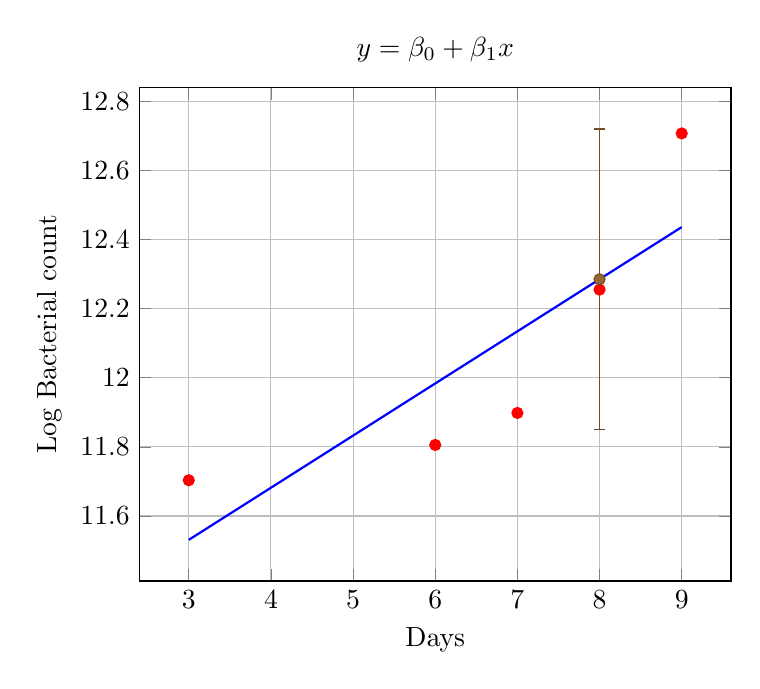
\begin{tikzpicture}
			\begin{axis}[width = 0.75\textwidth,xlabel=Days, ylabel=Log Bacterial count, grid=both, title = {$y = \beta_0 + \beta_1 x$}]
				\addplot[thick, smooth, draw=blue][domain=3:9]{0.1508*x + 11.0787};
				\addplot[only marks, color = red] plot coordinates{(3, 11.703545824578878) (6, 11.805595078933049) (7, 11.898187865760873) (8, 12.254862809699606) (9, 12.706847933442663)};
				\addplot+[mark = *, error bars/.cd, y dir=both,y explicit] coordinates{ (8, 12.284890664087893) +- (0, 0.43478189254625227)  };
			\end{axis}
		\end{tikzpicture}
	\end{subfigure}
\end{figure}

\item Performing the polynomial regression using custom script outputs \\


\begin{figure}[H]
	\begin{subfigure}[]{0.2\linewidth}
		\centering
		\begin{tabular}{@{}rr@{}}
			\toprule
			\multicolumn{2}{c}{\texttt{PolyRegressOutput}} \\
			\midrule
			$\beta_0$ &           1.8300 \\
			$\beta_1$ &          -0.3398 \\
			$\beta_2$ &           0.0267 \\
			\bottomrule
		\end{tabular}
		
	\end{subfigure}
	%
	\begin{subfigure}[]{0.8\linewidth}
		\centering
		
		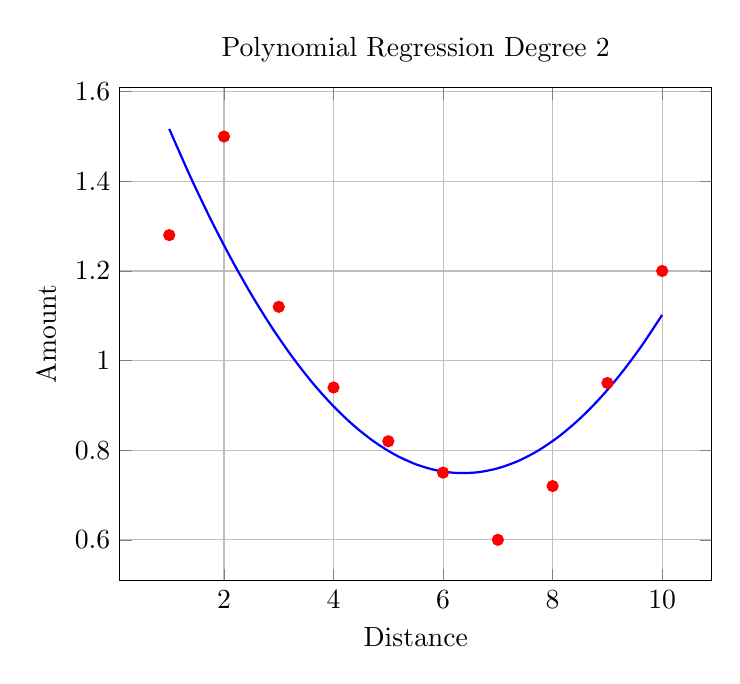
\begin{tikzpicture}
			\begin{axis}[width = 0.75\textwidth,xlabel=Distance, ylabel=Amount, grid=both, title = {Polynomial Regression Degree 2 }]
				\addplot[thick, smooth, draw=blue][domain=1.0:10.0]{1.83 - 0.3398*x^1 + 0.0267*x^2};
				\addplot[only marks, color = red] plot coordinates{(1.0, 1.28) (2.0, 1.5) (3.0, 1.12) (4.0, 0.94) (5.0, 0.82) (6.0, 0.75) (7.0, 0.6) (8.0, 0.72) (9.0, 0.95) (10.0, 1.2)};
			\end{axis}
		\end{tikzpicture}
	\end{subfigure}
\end{figure}

\item Performing the polynomial regression using custom script outputs \\

\begin{figure}[H]
	\begin{subfigure}[]{0.2\linewidth}
		\centering
		\begin{tabular}{@{}rr@{}}
			\toprule
			\multicolumn{2}{c}{\texttt{PolyRegressOutput}} \\
			\midrule
			$\beta_0$ &          -0.0283 \\
			$\beta_1$ &           0.5515 \\
			$\beta_2$ &          -0.0473 \\
			\bottomrule
		\end{tabular}
		
	\end{subfigure}
	%
	\begin{subfigure}[]{0.8\linewidth}
		\centering
		
		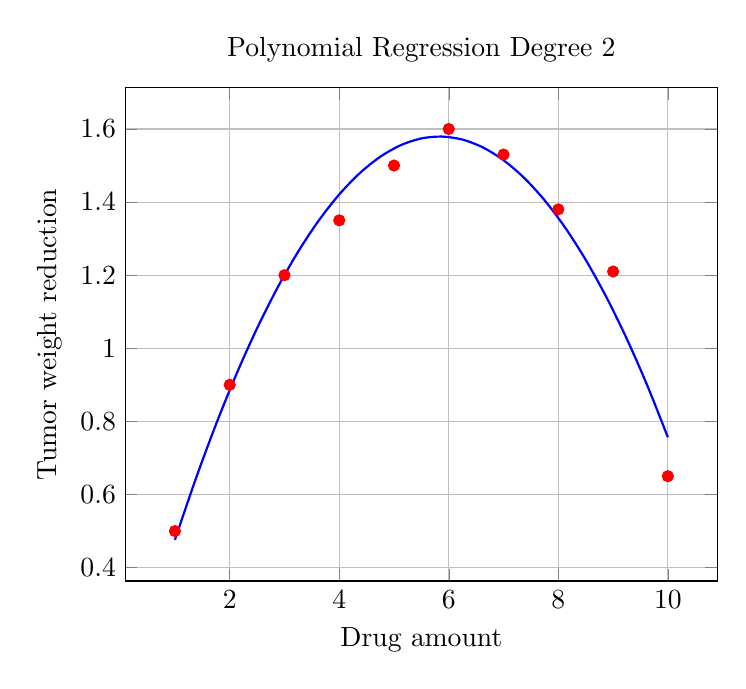
\begin{tikzpicture}
			\begin{axis}[width = 0.75\textwidth,xlabel=Drug amount, ylabel=Tumor weight reduction, grid=both, title = {Polynomial Regression Degree 2 }]
				\addplot[thick, smooth, draw=blue][domain=1:10]{-0.0283 + 0.5515*x^1 - 0.0473*x^2};
				\addplot[only marks, color = red] plot coordinates{(1, 0.5) (2, 0.9) (3, 1.2) (4, 1.35) (5, 1.5) (6, 1.6) (7, 1.53) (8, 1.38) (9, 1.21) (10, 0.65)};
			\end{axis}
		\end{tikzpicture}
	\end{subfigure}
\end{figure}


\item Starting with linear regression gives,

\begin{figure}[H]
	\begin{subfigure}[]{0.2\linewidth}
		\centering
		\begin{tabular}{@{}rr@{}}
			\toprule
			\multicolumn{2}{c}{\texttt{PolyRegressOutput}} \\
			\midrule
			$\beta_0$ &         -46.5405 \\
			$\beta_1$ &          32.0270 \\
			\bottomrule
		\end{tabular}
		
	\end{subfigure}
	%
	\begin{subfigure}[]{0.8\linewidth}
		\centering
		
		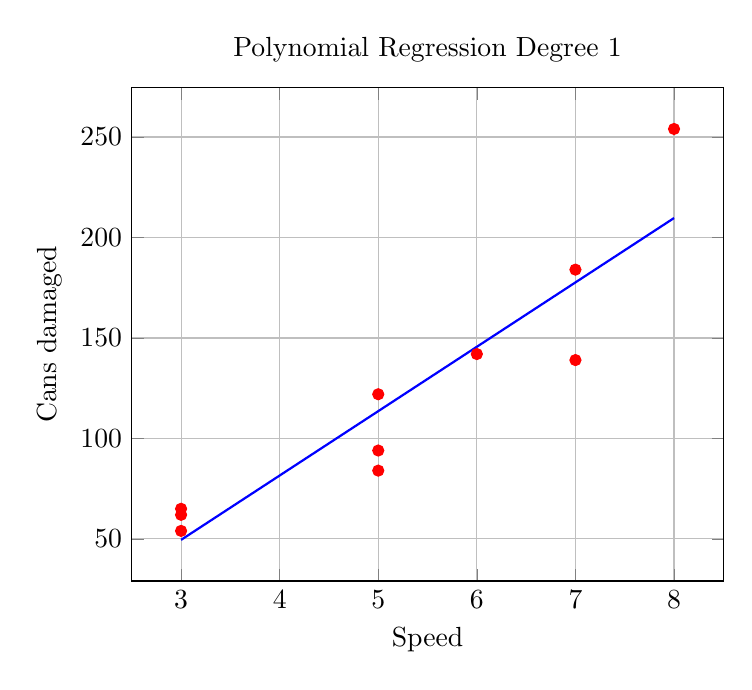
\begin{tikzpicture}
			\begin{axis}[width = 0.75\textwidth,xlabel=Speed, ylabel=Cans damaged, grid=both, title = {Polynomial Regression Degree 1 }]
				\addplot[thick, smooth, draw=blue][domain=3:8]{-46.5405 + 32.027*x^1};
				\addplot[only marks, color = red] plot coordinates{(3, 54) (3, 62) (3, 65) (5, 94) (5, 122) (5, 84) (6, 142) (7, 139) (7, 184) (8, 254)};
			\end{axis}
		\end{tikzpicture}
	\end{subfigure}
\end{figure}

Plotting the standardized residuals \\

\begin{figure}[H]
	\centering
	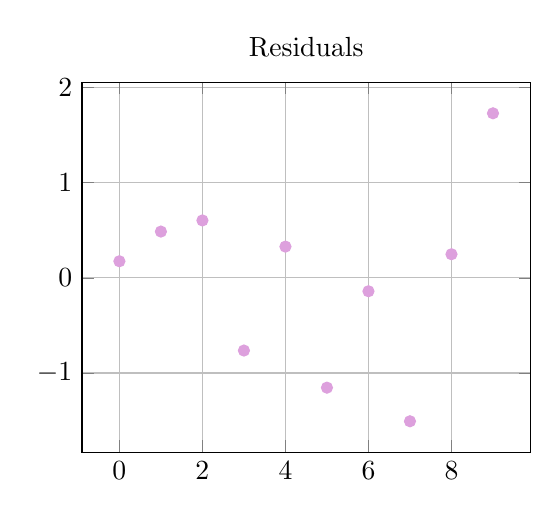
\begin{tikzpicture}
		\begin{axis}[width = 0.6\textwidth, grid=both, title = {Residuals}]
			\addplot[only marks, color = Plum] plot coordinates{(0, 0.1739738216124868) (1, 0.48607231371730614) (2, 0.6031092482566134) (3, -0.7644304282972766) (4, 0.32791429406959105) (5, -1.1545535434283007) (6, -0.14128783088528954) (7, -1.5077731206415268) (8, 0.24778089744808193) (9, 1.7291943481483212)};
		\end{axis}
	\end{tikzpicture}
\end{figure}

Trying out a degree 2 polynomial regression gives a better looking result.

\begin{figure}[H]
	\begin{subfigure}[]{0.2\linewidth}
		\centering
		\begin{tabular}{@{}rr@{}}
			\toprule
			\multicolumn{2}{c}{\texttt{PolyRegressOutput}} \\
			\midrule
			$\beta_0$ &         101.4700 \\
			$\beta_1$ &         -31.3477 \\
			$\beta_2$ &           6.0513 \\
			\bottomrule
		\end{tabular}
		
	\end{subfigure}
	%
	\begin{subfigure}[]{0.8\linewidth}
		\centering
		
		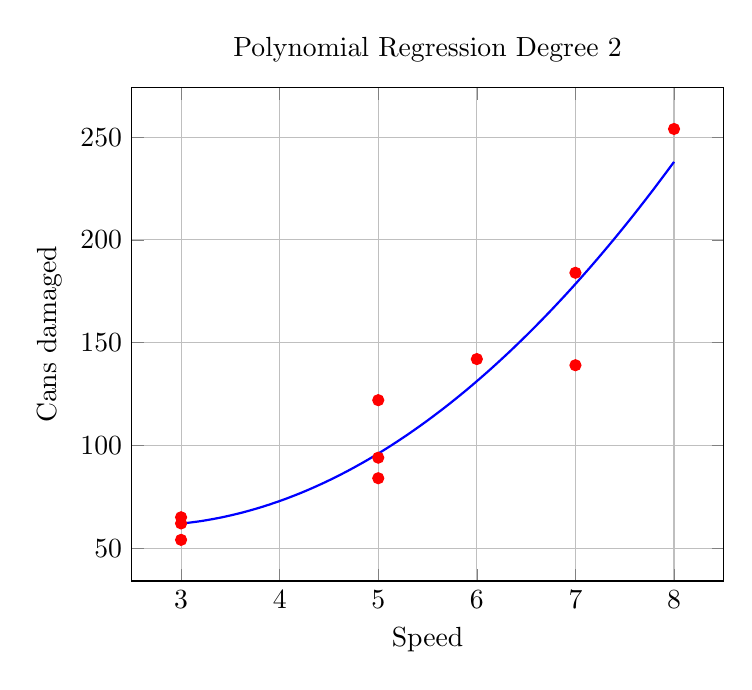
\begin{tikzpicture}
			\begin{axis}[width = 0.75\textwidth,xlabel=Speed, ylabel=Cans damaged, grid=both, title = {Polynomial Regression Degree 2 }]
				\addplot[thick, smooth, draw=blue][domain=3:8]{101.47 - 31.3477*x^1 + 6.0513*x^2};
				\addplot[only marks, color = red] plot coordinates{(3, 54) (3, 62) (3, 65) (5, 94) (5, 122) (5, 84) (6, 142) (7, 139) (7, 184) (8, 254)};
			\end{axis}
		\end{tikzpicture}
	\end{subfigure}
\end{figure}

\item Performing linear regression, but with variance in $ Y $ proportional to $ x $,

\begin{align}
	\mathrm{Var}(Y_i) &= \frac{\sigma^2}{w_i} \nonumber \\
	%
	w_i &\propto \frac{1}{x_i}
\end{align}

\begin{figure}[H]
	\begin{subfigure}[]{0.2\linewidth}
		\centering
		\begin{tabular}{@{}rr@{}}
			\toprule
			\multicolumn{2}{c}{\texttt{PolyRegressOutput}} \\
			\midrule
			$\beta_0$ &           0.5250 \\
			$\beta_1$ &          12.1434 \\
			\bottomrule
		\end{tabular}
		
	\end{subfigure}
	%
	\begin{subfigure}[]{0.8\linewidth}
		\centering
		
		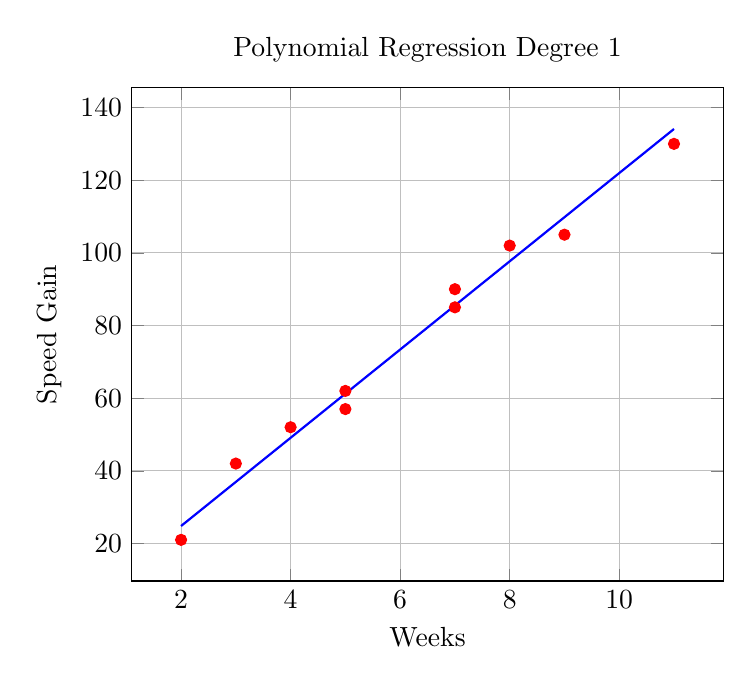
\begin{tikzpicture}
			\begin{axis}[width = 0.75\textwidth,xlabel=Weeks, ylabel=Speed Gain, grid=both, title = {Polynomial Regression Degree 1 }]
				\addplot[thick, smooth, draw=blue][domain=2:11]{0.525 + 12.1434*x^1};
				\addplot[only marks, color = red] plot coordinates{(2, 21) (3, 42) (8, 102) (11, 130) (4, 52) (5, 57) (9, 105) (7, 85) (5, 62) (7, 90)};
			\end{axis}
		\end{tikzpicture}
	\end{subfigure}
\end{figure}

\item Performing the polynomial regression with degree 2 using custom script outputs \\
The value corresponding to $ x = 42 $ is $ y = 0.3429 $.

\begin{figure}[H]
	\begin{subfigure}[]{0.2\linewidth}
		\centering
		\begin{tabular}{@{}rr@{}}
			\toprule
			\multicolumn{2}{c}{\texttt{PolyRegressOutput}} \\
			\midrule
			$\beta_0$ &          -0.0015 \\
			$\beta_1$ &          -0.0002 \\
			$\beta_2$ &           0.0002 \\
			\bottomrule
		\end{tabular}
		
	\end{subfigure}
	%
	\begin{subfigure}[]{0.8\linewidth}
		\centering
		
		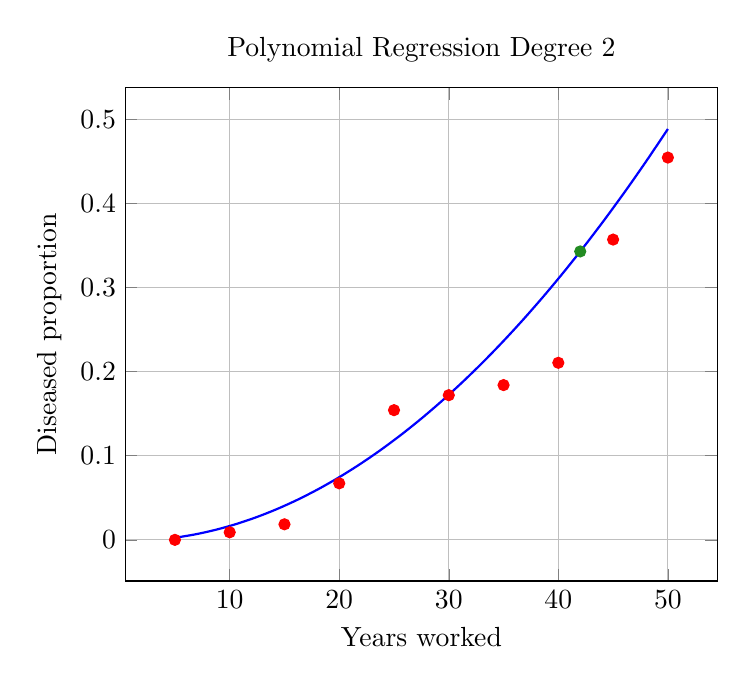
\begin{tikzpicture}
			\begin{axis}[width = 0.75\textwidth,xlabel=Years worked, ylabel=Diseased proportion, grid=both, title = {Polynomial Regression Degree 2 }]
				\addplot[thick, smooth, draw=blue][domain=5:50]{-0.0015 - 0.0002*x^1 + 0.0002*x^2};
				\addplot[only marks, color = red] plot coordinates{(5, 0.0) (10, 0.009) (15, 0.0185) (20, 0.0672) (25, 0.1542) (30, 0.172) (35, 0.184) (40, 0.2105) (45, 0.357) (50, 0.4545)};
				\addplot[only marks, color = ForestGreen] plot coordinates{ (42, 0.3429) };
			\end{axis}
		\end{tikzpicture}
	\end{subfigure}
\end{figure}


\item Performing linear regression, but with variance in $ Y $ proportional to $ x $,
The value corresponding to $ x = 3500 $ is $ y = 31.4 $.

\begin{figure}[H]
	\begin{subfigure}[]{0.2\linewidth}
		\centering
		\begin{tabular}{@{}rr@{}}
			\toprule
			\multicolumn{2}{c}{\texttt{PolyRegressOutput}} \\
			\midrule
			$\beta_0$ &          -4.6584 \\
			$\beta_1$ &           0.0103 \\
			\bottomrule
		\end{tabular}
		
	\end{subfigure}
	%
	\begin{subfigure}[]{0.8\linewidth}
		\centering
		
		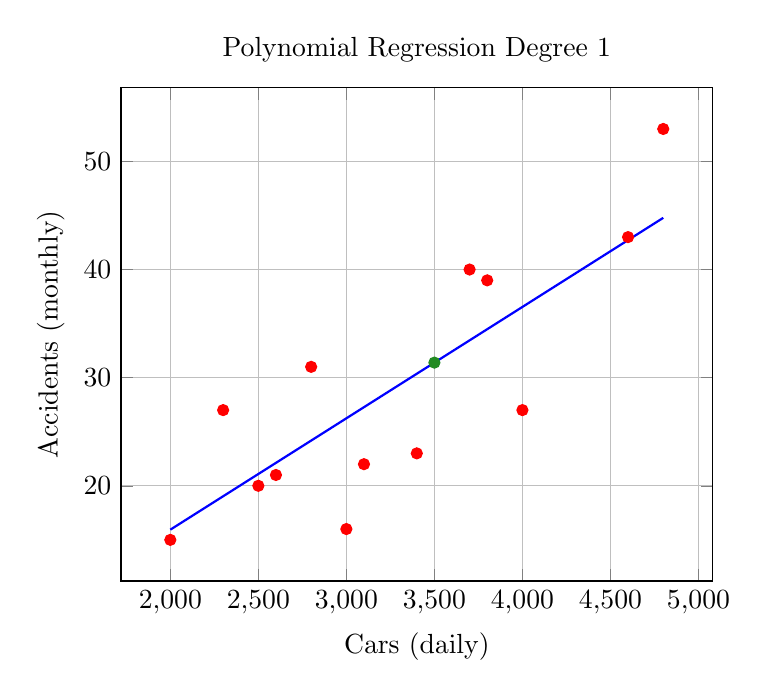
\begin{tikzpicture}
			\begin{axis}[width = 0.75\textwidth,xlabel=Cars (daily), ylabel=Accidents (monthly), grid=both, title = {Polynomial Regression Degree 1 }]
				\addplot[thick, smooth, draw=blue][domain=2000:4800]{-4.6584 + 0.0103*x^1};
				\addplot[only marks, color = red] plot coordinates{(2000, 15) (2300, 27) (2500, 20) (2600, 21) (2800, 31) (3000, 16) (3100, 22) (3400, 23) (3700, 40) (3800, 39) (4000, 27) (4600, 43) (4800, 53)};
				\addplot[only marks, color = ForestGreen] plot coordinates{ (3500, 31.3916) };
			\end{axis}
		\end{tikzpicture}
	\end{subfigure}
\end{figure}

Redoing the problem with $ \sqrt{Y} = \beta_0 + \beta_1 x + e $,
The value corresponding to $ x = 3500 $ is $ \sqrt{Y} = 5.3725 $ which corresponds to $ Y = 28.86 $.

\begin{figure}[H]
	\begin{subfigure}[]{0.2\linewidth}
		\centering
		\begin{tabular}{@{}rr@{}}
			\toprule
			\multicolumn{2}{c}{\texttt{PolyRegressOutput}} \\
			\midrule
			$\beta_0$ &           2.2225 \\
			$\beta_1$ &           0.0009 \\
			\bottomrule
		\end{tabular}
		
	\end{subfigure}
	%
	\begin{subfigure}[]{0.8\linewidth}
		\centering
		
		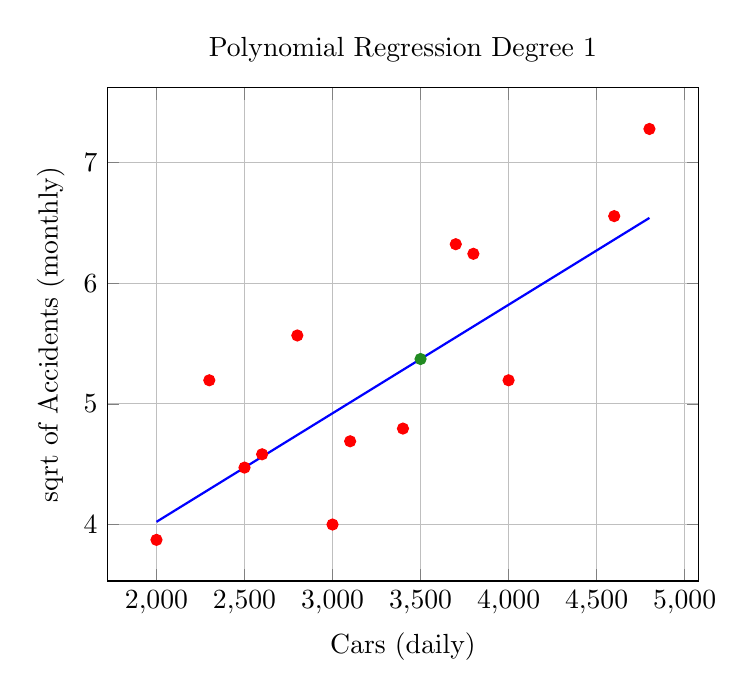
\begin{tikzpicture}
			\begin{axis}[width = 0.75\textwidth,xlabel=Cars (daily), ylabel={sqrt of Accidents (monthly)}, grid=both, title = {Polynomial Regression Degree 1 }]
				\addplot[thick, smooth, draw=blue][domain=2000:4800]{2.2225 + 0.0009*x^1};
				\addplot[only marks, color = red] plot coordinates{(2000, 3.872983346207417) (2300, 5.196152422706632) (2500, 4.47213595499958) (2600, 4.58257569495584) (2800, 5.5677643628300215) (3000, 4.0) (3100, 4.69041575982343) (3400, 4.795831523312719) (3700, 6.324555320336759) (3800, 6.244997998398398) (4000, 5.196152422706632) (4600, 6.557438524302) (4800, 7.280109889280518)};
				\addplot[only marks, color = ForestGreen] plot coordinates{ (3500, 5.3725) };
			\end{axis}
		\end{tikzpicture}
	\end{subfigure}
\end{figure}

\item Using custom multiple linear regression with 2 inputs,

\begin{figure}[H]
	\centering
	\begin{tabular}{@{}rr@{}}
		\toprule
		\multicolumn{2}{c}{\texttt{MultiLinRegressOutput}} \\
		\midrule
		$\beta_0$ &         150.1414 \\
		$\beta_1$ &           0.3621 \\
		$\beta_2$ &       -3163.5648 \\
		\bottomrule
	\end{tabular}
	
\end{figure}

\item Using custom multiple linear regression with 2 inputs,

\begin{figure}[H]
	\centering
	\begin{tabular}{@{}rr@{}}
		\toprule
		\multicolumn{2}{c}{\texttt{MultiLinRegressOutput}} \\
		\midrule
		$\beta_0$ &          -1.5962 \\
		$\beta_1$ &           0.2662 \\
		$\beta_2$ &           0.0004 \\
		\bottomrule
	\end{tabular}
	
\end{figure}

\item Using custom multiple linear regression with inputs 2, 3 and 4 (input 1 is ignored because of collinearity with input 2 as seen in the correlation matrix),

\begin{figure}[H]
	\centering
	  \renewcommand{\arraystretch}{2}
	\begin{tabular}{lrrrr}
		\toprule
		 &      x1 &      x2 &      x3 &      x4 \\
		\midrule
		x1 &  1.0000 &  1.0000 &  0.3725 &  0.9947 \\
		x2 &  1.0000 &  1.0000 &  0.3725 &  0.9947 \\
		x3 &  0.3725 &  0.3725 &  1.0000 &  0.3986 \\
		x4 &  0.9947 &  0.9947 &  0.3986 &  1.0000 \\
		\bottomrule
	\end{tabular}
\end{figure}

With the collinear variables removed and the model dimensions reduced to $ \{x_2, x_3, x_4\} $,

\begin{figure}[H]
	\centering
	\begin{tabular}{@{}rr@{}}
		\toprule
		\multicolumn{2}{c}{\texttt{MultiLinRegressOutput}} \\
		\midrule
		$\beta_0$ &          18.6060 \\
		$\beta_2$ &           9.9179 \\
		$\beta_3$ &          14.0753 \\
		$\beta_4$ &         -19.1818 \\
		\bottomrule
	\end{tabular}
\end{figure}


\item Using custom multiple linear regression with 2 inputs and log response as output,

\begin{figure}[H]
	\centering
	\begin{tabular}{@{}rr@{}}
		\toprule
		\multicolumn{2}{c}{\texttt{MultiLinRegressOutput}} \\
		\midrule
		$\beta_0$ &           7.9567 \\
		$\beta_1$ &          -1.2047 \\
		$\beta_2$ &          -0.0225 \\
		\bottomrule
	\end{tabular}
\end{figure}

The $ SS_R $ is 22.08, and using $ n = 12, k = 2 $, $ \sigma^2 = 2.453 $.

\item Using custom multiple linear regression with 3 inputs,

\begin{figure}[H]
	\centering
	\begin{tabular}{@{}rr@{}}
		\toprule
		\multicolumn{2}{c}{\texttt{MultiLinRegressOutput}} \\
		\midrule
		$\beta_0$ &          -2.8278 \\
		$\beta_1$ &           5.3707 \\
		$\beta_2$ &           9.8157 \\
		$\beta_3$ &           0.4482 \\
		\bottomrule
	\end{tabular}
	
\end{figure}

$ SS_R = 201.97 $ and the variance in response is $ \sigma^2 = 18.361 $\\
$ H_0 : \beta_0 = 0 $ has uses a t-test and has a p-value of 45.88\% \\
$ H_0 : \beta_3 = 0 $ has uses a t-test and has a p-value of 36.72\% \\
$ H_0 : 8.5 = \beta_0 + \beta_1 + \beta_2 + \beta_3 $ uses a t-test and has a p-value of 36.72\% \\

\begin{align}
	\ddfrac{\sum\limits_{i = 0}^{k} B_i x_i - \sum\limits_{i = 0}^{k} \beta_i x_i}{\sqrt{\textbf{x}^\intercal \ (\textbf{X}^\intercal \textbf{X})^{-1}\ \textbf{x}\ \left(\frac{SS_R}{n-k-1}\right)}} &\sim t_{n-k-1}
\end{align}

\item  Performing multiple regression using custom script with 2 inputs\\

\begin{figure}[H]
	\centering
	\begin{tabular}{@{}rr@{}}
		\toprule
		\multicolumn{2}{c}{\texttt{MultiLinRegressOutput}} \\
		\midrule
		$\beta_0$ &         177.6954 \\
		$\beta_1$ &           1.0351 \\
		$\beta_2$ &          10.7214 \\
		\bottomrule
	\end{tabular}
\end{figure}

The $ 90\% $ confidence interval for $ \{x_1 = 21, x_2 = 3.6\} $ is
$ 238.03 \pm 3.961 = [234.069, 241.991]$

\item Using custom multiple linear regression with 3 inputs,
$ SS_R = 4614.65 $ and $ \sigma^2 \approx 769.11 $

\begin{figure}[H]
	\centering
	\begin{tabular}{@{}rr@{}}
		\toprule
		\multicolumn{2}{c}{\texttt{MultiLinRegressOutput}} \\
		\midrule
		$\beta_0$ &        1108.7245 \\
		$\beta_1$ &           8.6393 \\
		$\beta_2$ &           0.2608 \\
		$\beta_3$ &          -0.7114 \\
		\bottomrule
	\end{tabular}
	
\end{figure}

The $ 95\% $ confidence interval for $ \{x_1 = 125, x_2 = 900, x_3 = 160\} $ is
$ 2309.51 \pm 37.85 = [2271.66, 2347.36]$

\item Same mean and larger variance of the prediction interval means that it is always going to larger than the mean response interval for the same confidence value.

\item Using custom multiple linear regression with 2 inputs,
$ SS_R = 619.43 $ and $ \sigma^2 \approx 68.825 $
\begin{figure}[H]
	\centering
	\begin{tabular}{@{}rr@{}}
		\toprule
		\multicolumn{2}{c}{\texttt{MultiLinRegressOutput}} \\
		\midrule
		$\beta_0$ &           5.2387 \\
		$\beta_1$ &           5.6968 \\
		$\beta_2$ &           9.5501 \\
		\bottomrule
	\end{tabular}
\end{figure}

The $ 95\% $ confidence interval for the predicted response at $ \{x_1 = 10.2, x_2 = 17\} $ is
$ 225.7 \pm 20.05 = [205.65, 245.75]$


\item Using custom multiple linear regression with 2 inputs,
$ SS_R = 0.5793 $ and $ \sigma^2 \approx 0.0644 $ \\
The hypothesis $ H_0 : \beta_1 = 0$ has a p-value 0.45\% using a t-test. The hypothesis can be safely rejected.



\begin{figure}[H]
	\centering
	\begin{tabular}{@{}rr@{}}
		\toprule
		\multicolumn{2}{c}{\texttt{MultiLinRegressOutput}} \\
		\midrule
		$\beta_0$ &           6.1439 \\
		$\beta_1$ &          -0.0376 \\
		$\beta_2$ &           0.0850 \\
		\bottomrule
	\end{tabular}
	
\end{figure}

The $ 95\% $ confidence interval for the predicted response at $ \{x_1 = 85, x_2 = 20\} $ is
$ 4.645 \pm 0.613 = [4.032, 5.259]$ \\

\item Using custom multiple linear regression with 2 inputs,
The hypothesis $ H_0 : \beta_1 = 0$ has a p-value 81\% using a t-test. The hypothesis cannot be rejected.

\begin{figure}[H]
	\centering
	\begin{tabular}{@{}rr@{}}
		\toprule
		\multicolumn{2}{c}{\texttt{MultiLinRegressOutput}} \\
		\midrule
		$\beta_0$ &          28.2098 \\
		$\beta_1$ &           0.1164 \\
		$\beta_2$ &           0.5664 \\
		\bottomrule
	\end{tabular}
	
\end{figure}

The $ 95\% $ confidence interval for the mean response at $ \{x_1 = 45, x_2 = 180\} $ is
$ 135.41 \pm 17.18 = [118.22, 152.59]$ \\
The $ 95\% $ confidence prediction interval for the response at $ \{x_1 = 45, x_2 = 180\} $ is
$ 135.41 \pm 51.28 = [84.12, 186.69]$ \\


\item Using custom multiple linear regression with 2 inputs,
Since $ \beta_2  < 0$, years on the job increasing lead to lesser job satisfaction.

\begin{figure}[H]
	\centering
	\begin{tabular}{@{}rr@{}}
		\toprule
		\multicolumn{2}{c}{\texttt{MultiLinRegressOutput}} \\
		\midrule
		$\beta_0$ &          -1.2050 \\
		$\beta_1$ &           0.1619 \\
		$\beta_2$ &          -0.1128 \\
		\bottomrule
	\end{tabular}
	
\end{figure}

The $ 95\% $ confidence prediction interval for the response at $ \{x_1 = 56, x_2 = 5\} $ is
$ 7.3 \pm 1.397 = [5.9, 8.7]$ \\

\item Performing the linear regression using \texttt{scipy.stats.linregress} outputs \\

\begin{figure}[H]
	\begin{subfigure}[]{0.2\linewidth}
		\centering
		\begin{tabular}{@{}rr@{}}
			\toprule
			\multicolumn{2}{c}{\texttt{linRegressOutput}} \\
			\midrule
			$\beta_1$     &         0.110682 \\
			$\beta_0$ &         5.636108 \\
			$r$    &         0.759205 \\
			$p$    &         0.017660 \\
			\bottomrule
		\end{tabular}
		
	\end{subfigure}
	%
	\begin{subfigure}[]{0.8\linewidth}
		\centering
		
		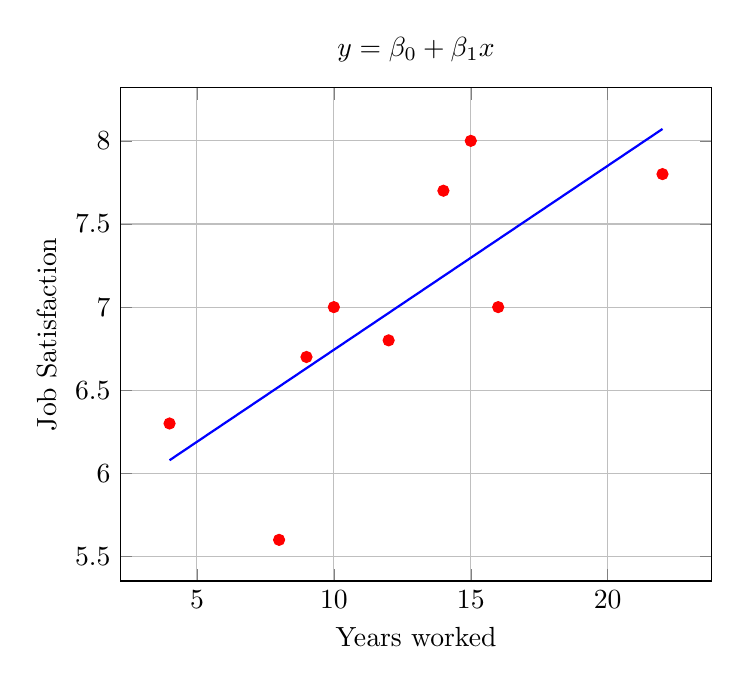
\begin{tikzpicture}
			\begin{axis}[width = 0.75\textwidth,xlabel=Years worked, ylabel=Job Satisfaction, grid=both, title = {$y = \beta_0 + \beta_1 x$}]
				\addplot[thick, smooth, draw=blue][domain=4.0:22.0]{0.1107*x + 5.6361};
				\addplot[only marks, color = red] plot coordinates{(4.0, 6.3) (8.0, 5.6) (9.0, 6.7) (10.0, 7.0) (12.0, 6.8) (14.0, 7.7) (15.0, 8.0) (16.0, 7.0) (22.0, 7.8)};
			\end{axis}
		\end{tikzpicture}
	\end{subfigure}
\end{figure}

Since $ \beta_1  > 0$, years on the job increasing lead to greater job satisfaction.

The trend is reversed compared to the relationship between the same input and response in the presence of the other input variable.

The reversal in relationship between $ x_2 $ and $ y $ upon the introduction of $ x_1 $ happens because of significant multicollinearity, as seen in the correlation matrix.

\begin{figure}[H]
	\centering
	\renewcommand{\arraystretch}{2}
\begin{tabular}{lrr}
	\toprule
	{} &      x1 &       x2 \\
	\midrule
	x1 &  1.0000 &  0.7592 \\
	x2  &  0.7592 &  1.0000 \\
	\bottomrule
\end{tabular}
\end{figure}


\item To find the value of $ x $ corresponding to $ p(x) = 0.5 $\\

\begin{align}
	p(x) &= \frac{\exp(a + bx)}{1 + \exp(a + bx)} = 0.5 \nonumber \\
	%
	\frac{y}{1 + y} &= \frac{1}{2} \nonumber \\
	%
	y &= 1 = \exp (a + bx) \nonumber \\
	%
	x^* &= -\frac{a}{b}
\end{align}

\item How to do logistic regression

\item How to do logistic regression



\end{enumerate}

